\chapter{\chapiiname}
\label{chapter2}
Humans can complete complex tasks due to their intelligence, dexterity, and physical make up. These complex tasks include agricultural picking, culinary preparation, factory goods processing, and biomedical practice. To complete these tasks with machines it is important to quantify these human qualities that the technology must match of supersede. The first part of this section is focused on understanding and quantifying human skin and muscle tissue often required for these complex human tasks. In parallel, artificial skin and artificial muscle state-of-the-art technology is reviewed. Finally, background theory on piezoresistive elastomer composites which will be utilised with specific sensor and actuator technology is given to setup foundational knowledge base and reference for the rest of the thesis.


    
\section{Biological Skin form and function}
Skin is the largest organ in the human body with many functions, however this thesis only aims to replicate some pressure-sensitive functions of skin. Two pressure-sensitive categories of skin and muscle tissue transducers which allow for dexterous manipulation of objects are:
\begin{enumerate} 
    \item Proprioceptors: respond to internal mechanical stimuli in a joint capsule, tendon, or muscle to give the sense of motion.
    \item Cutaneous mechanoreceptors:  respond to mechanical stimuli usually external to the body, including pressure and vibration, for the localisation of sensations. 
\end{enumerate} 
Locations of both proprioceptors and cutaneous mechanoreceptors are shown diagrammatically in Figure \ref{fig:proprioceptors-mechanoreceptors}. Proprioceptors aid in determining pose estimates of body parts in space, acting as sensors providing feedback closed-loop control for the neurological motion control of body parts. Whereas cutaneous mechanoreceptors have various roles including object recognition, manipulation control, as well as motion control.
\begin{figure}[H]
    \centering
    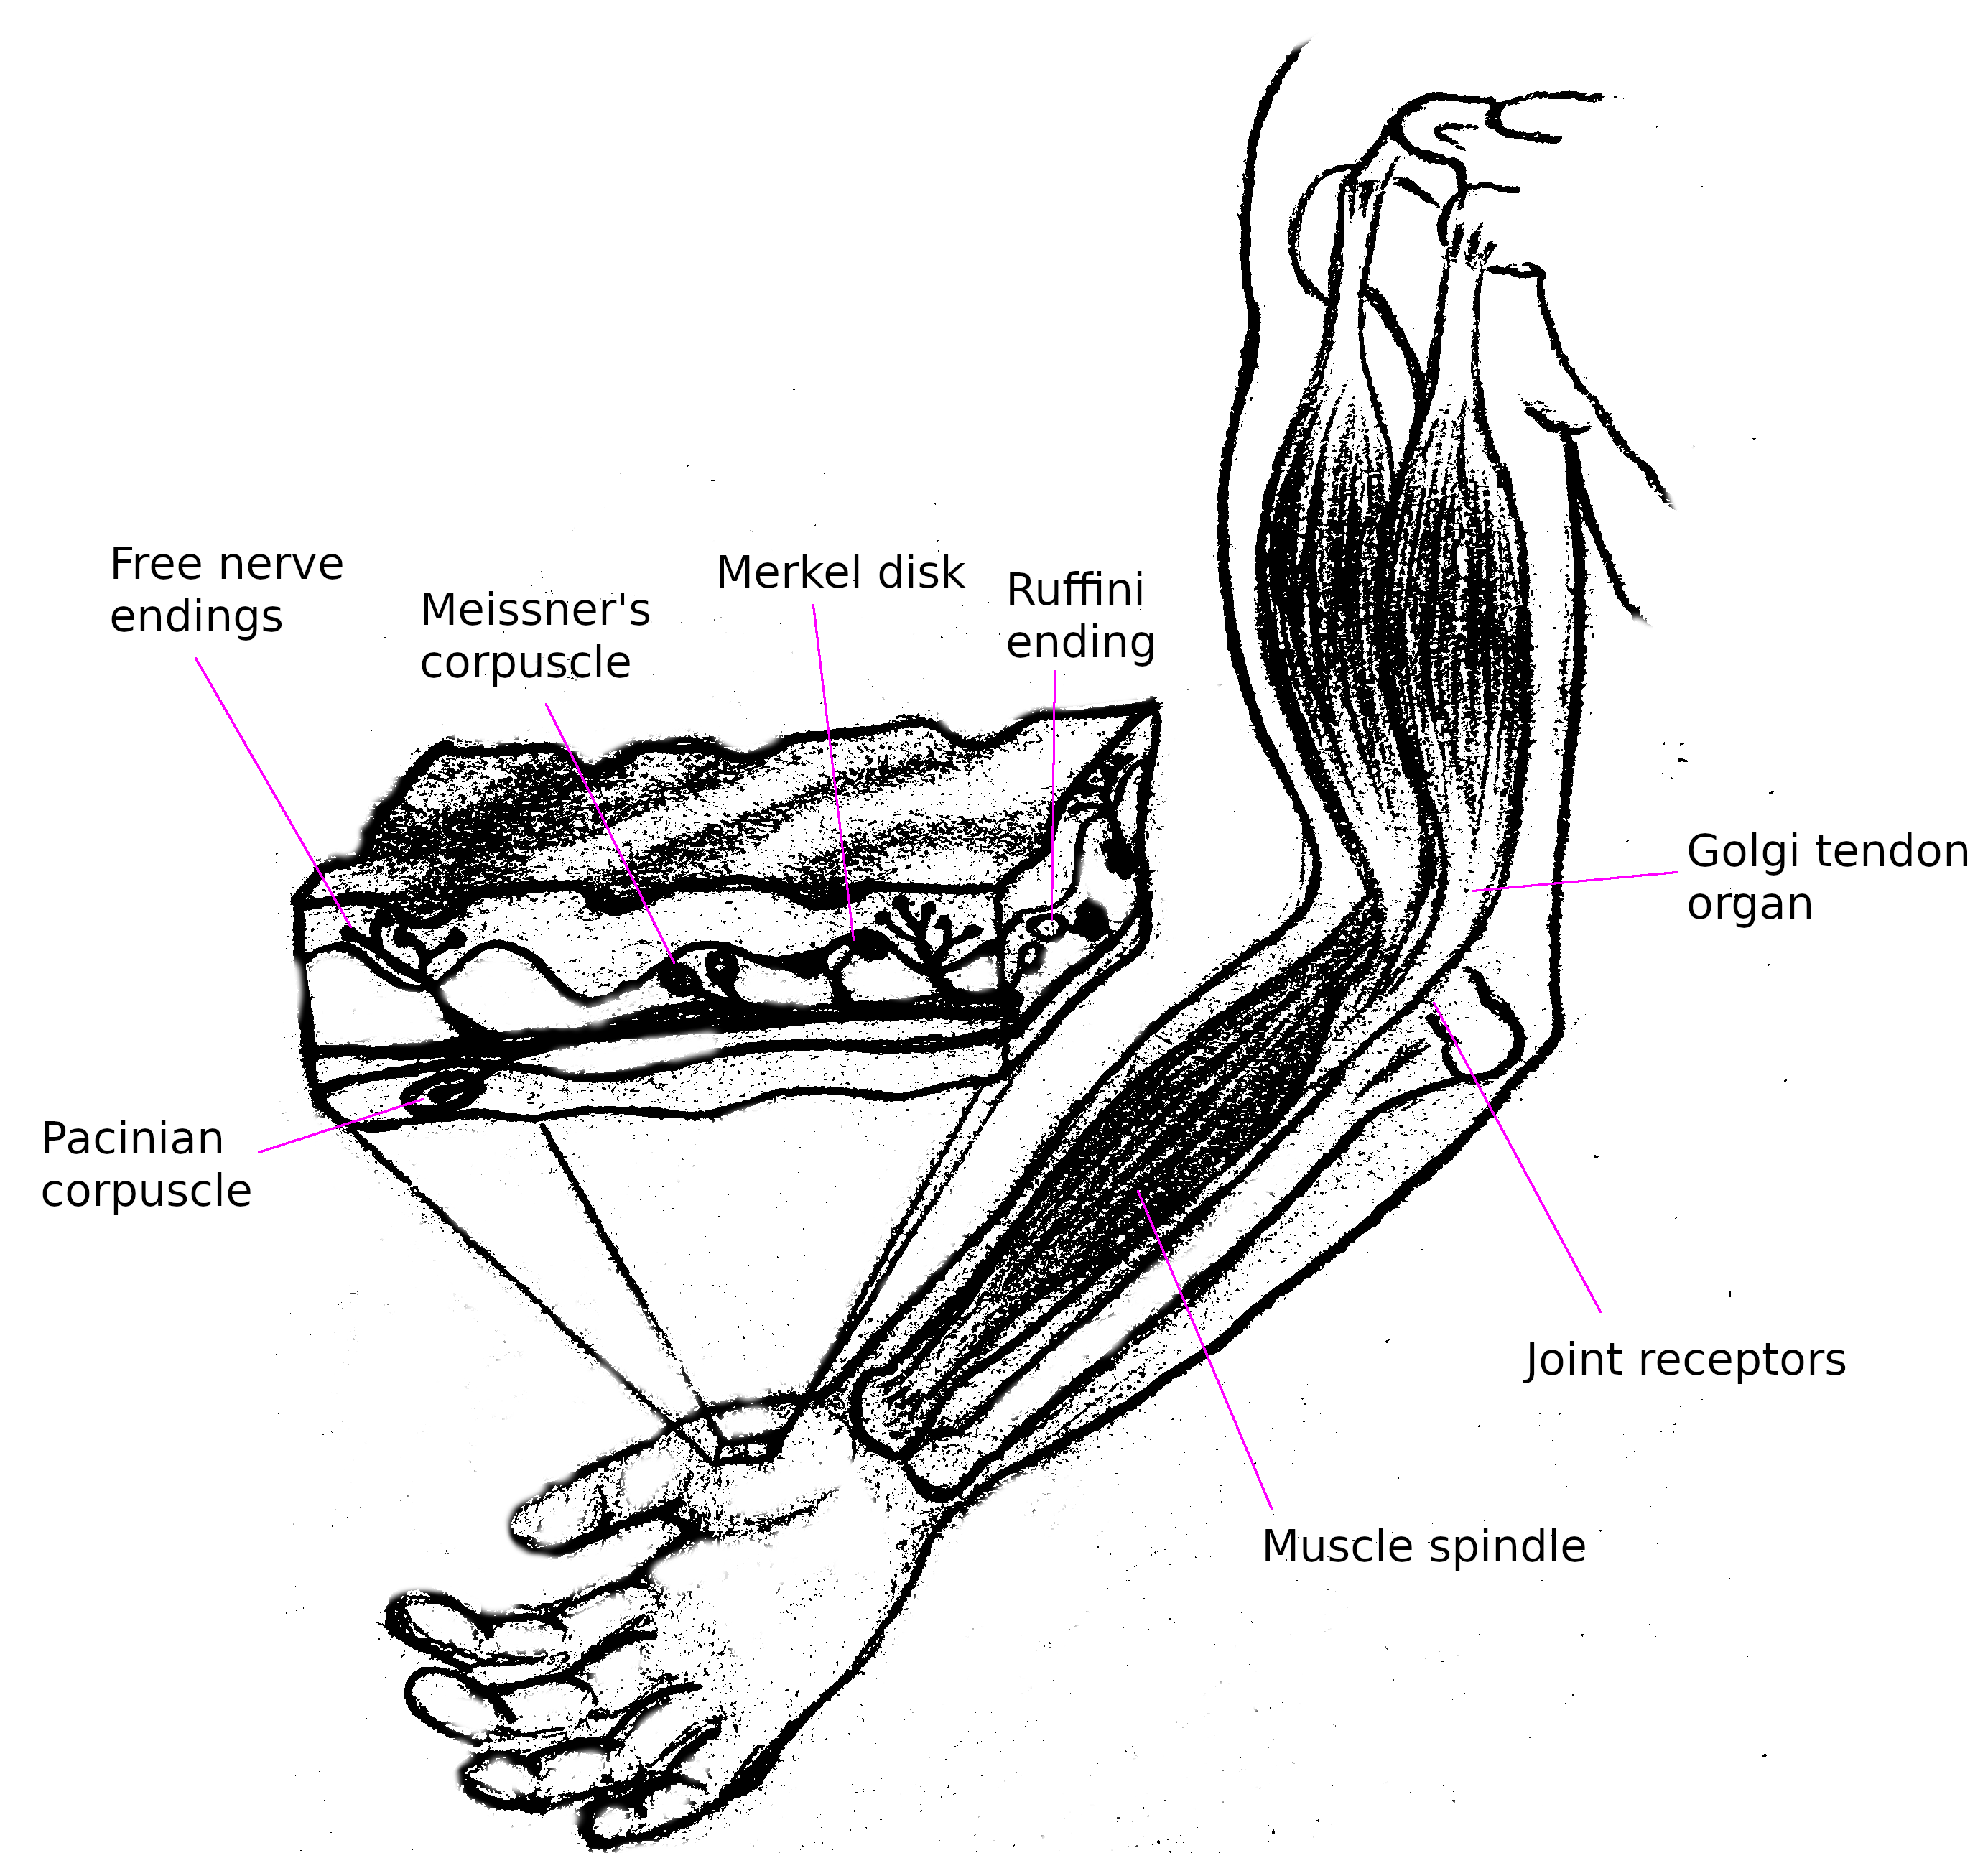
\includegraphics[width=0.6\linewidth]{Figures/propriocetors_n_cutaneous_mechanoreceptors_labelled.png}
    \caption{Examples of the locations of proprioceptors and cutaneous mechanoreceptors in the human body.}
    \label{fig:proprioceptors-mechanoreceptors}
\end{figure}

The function of both kinds of receptor have been mimicked by certain device technologies. For example proprioceptors have been mimicked in wearables and human assistive devices where joint motion has been estimated by sensors such as rotary/linear encoders, inertial measurement units (IMUs), and stretch sensors fixed adjacent to joints to calculate pose estimates of limbs\cite{OBrien2014,Eguchi2020,Chatfield2021,Kim2022}. Examples of such devices are displayed in Figure \ref{fig:proprio-tech}
%% Todo: Get copyright permission from image owners %%
\begin{figure}[H]
    \centering
    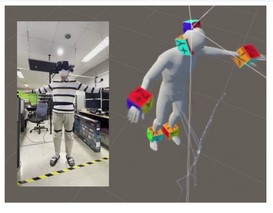
\includegraphics[width=0.4\linewidth]{Figures/imu-pose-tracker-kim2022.jpg} % no copyright permission required
    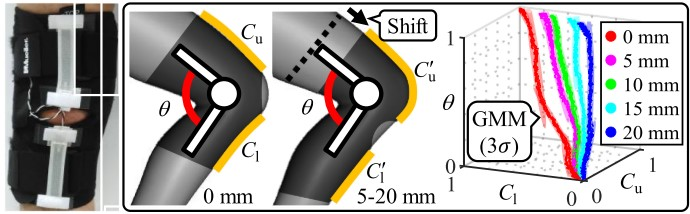
\includegraphics[width=0.4\linewidth]{Figures/knee-stretch-sense-eguchi2020.jpg} % 
    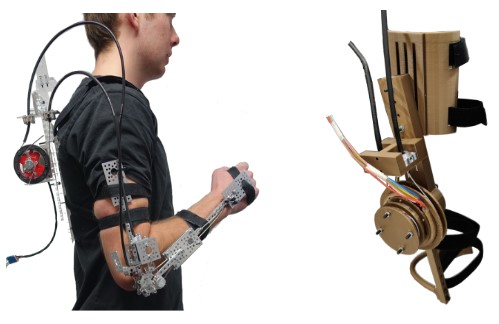
\includegraphics[width=0.4\linewidth]{Figures/logan-assitive-arm-device.jpg}
    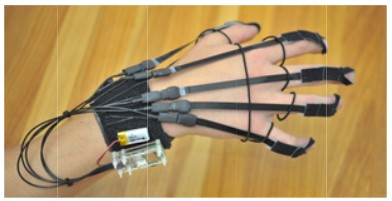
\includegraphics[width=0.4\linewidth]{Figures/stretch-sense-OBrien2014.jpg}
    \caption{Clockwise from top left: IMU pose estimation\cite{Kim2022} ($\copyright$ 2022 MDPI), stretch sensor knee joint pose estimation\cite{Eguchi2020} ($\copyright$ 2020 IEEE), encoder elbow pose joint estimation\cite{Chatfield2021}, stretch sensor hand joint pose estimations\cite{OBrien2014}.}
    \label{fig:proprio-tech}
\end{figure}
Cutaneous mechanoreceptors have been mimicked by the development of pressure mapping of flexible surfaces. Examples of such technologies include, foot pressure based gait analysis, wheelchair seat pressure mapping. Commercially available examples of these sensors are shown in Figure \ref{fig:mechano-tech}.
\begin{figure}[H]
    \centering
    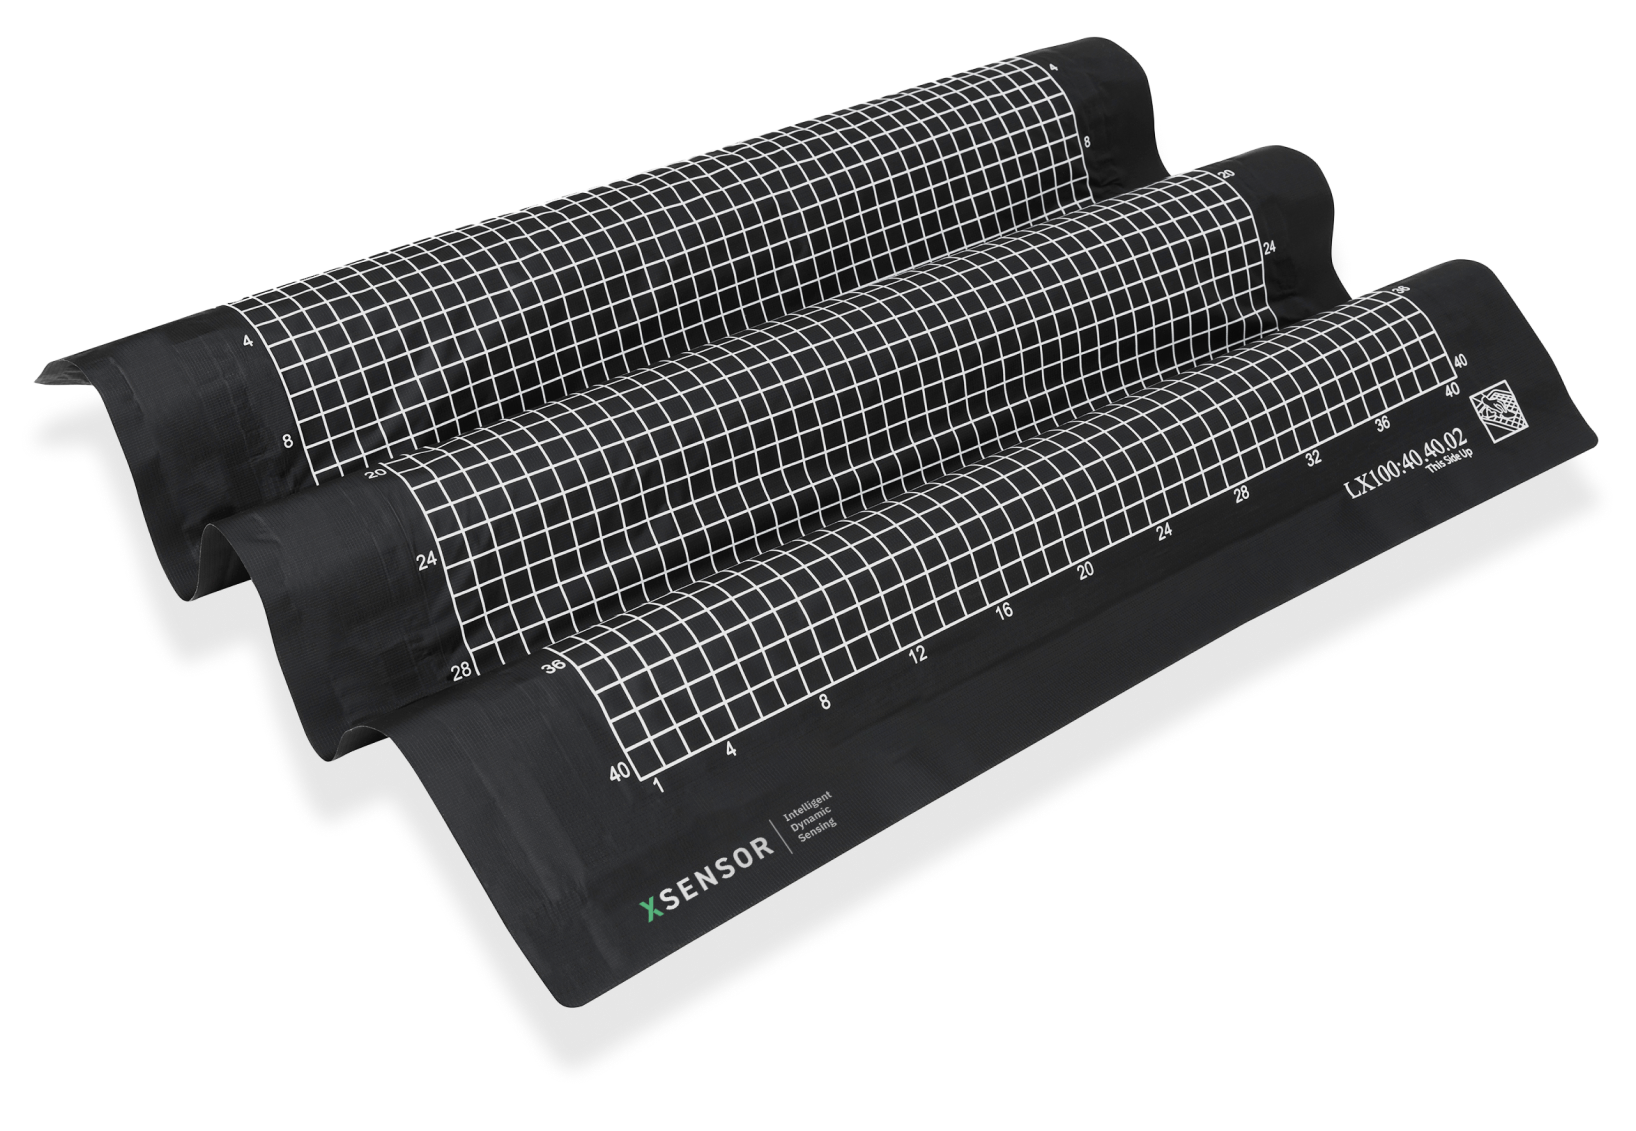
\includegraphics[width=0.4\linewidth]{Figures/xsensor.png}
    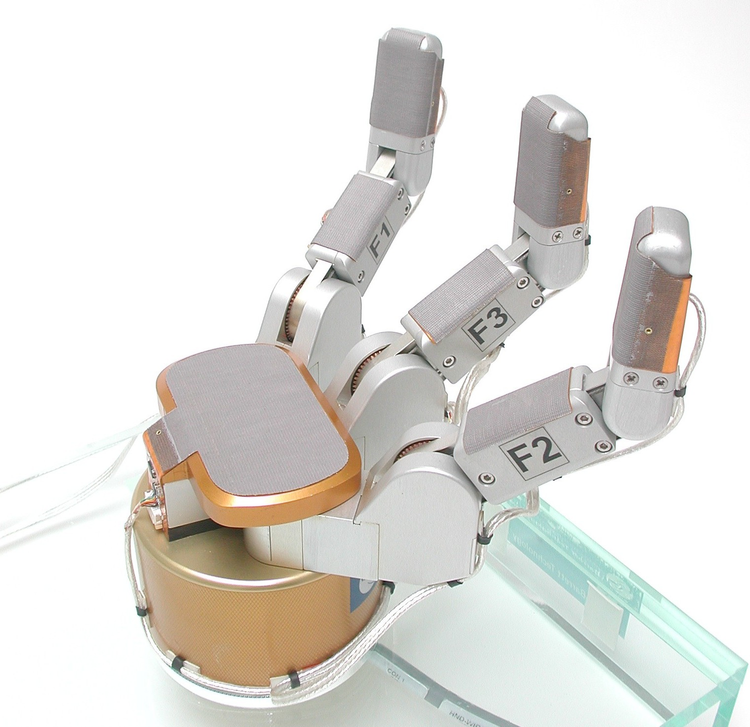
\includegraphics[width=0.4\linewidth]{Figures/Robotic+arm+with+PPS+sensors.png}
    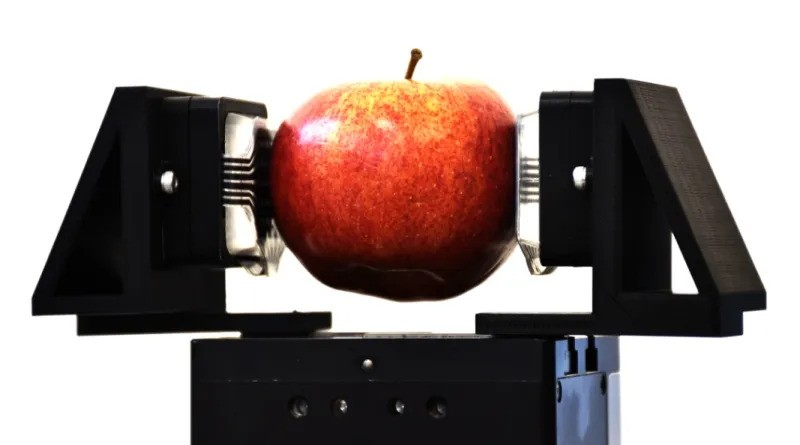
\includegraphics[width=0.4\linewidth]{Figures/powerOn_gripper_apple.jpg}
    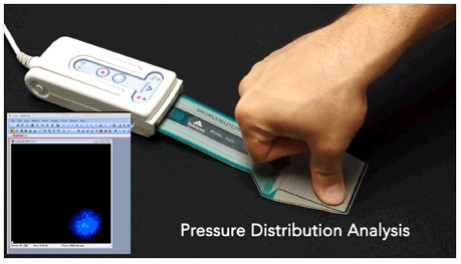
\includegraphics[width=0.4\linewidth]{Figures/tekscan-pressure-sensor.jpg} % only commercial image without permission granted.
    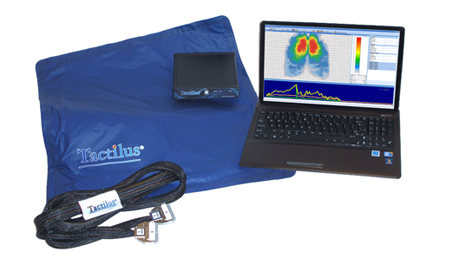
\includegraphics[width=0.4\linewidth]{Figures/tactilus-pressuremap-sensor-laptop.jpg}
    \caption{Various pressure mapping devices. From top-left then clockwise: XSsensor wheelchair pressure mapping sheet ($\copyright$ 2024 XSENSOR\textsuperscript{\textregistered} Technology)\cite{Xsensor}, Pressure Profile Systems pressure sensors on a robotic hand ($\copyright$ 2023 PPS UK limited)\cite{PressureProfile2023}, Soft pressure mapping gripper($\copyright$ 2023 PowerON)\cite{PowerOn}, Tekscan thin pressure mapping platform\cite{Tekscan}($\copyright$ 2024 Tekscan Inc.), Tactilus seat pressure mapping system\cite{SensorProducts}($\copyright$ 2024 Sensor Products Inc.)}

    \label{fig:mechano-tech}
\end{figure}
%% Todo: Get copyright permission from image owners %%
Many of these pressure mapping technologies don't accurately mimic desirable qualities of regular biological skin and are specialised for their specific use cases. The following sections quantify characteristics of pressure sensitive skin.

\subsection{Skin Construction and Types}
Skin is a laminate structure consisting of three main layers, the epidermis, dermis, and hypodermis. The top two layers the epidermis and dermis are a subset of the cutaneous layer which contain the majority of the pressure-sensitive mechanoreceptors \cite{McGrath2010}.

The skin can be categorised as glabrous/hairless or non-glabrous/hairy. Glabrous skin contains many of the mechanoreceptors given in Figure \ref{fig:proprioceptors-mechanoreceptors} whereas non-glabrous skin will also contain C-tactile afferent receptors for obtaining sensations through hair follicles. However this work is exploring simple monolithic/homogeneous-composite bodies so will not be replicating the sensor function of non-glabrous skin.

Depending on the region of skin different force resolution and spatial resolution will incur. Relevant cutaneous mechanoreceptors and their functions are given in Table \ref{tab:mechanoreceptors-table}. The tensile properties of skin is governed by skin tension lines, also called Lager's lines, which show the direction in which the maximal stretch can occur. 

%\begin{table}[H]
%    \centering
%    \caption{Comparison of typical mammalian mechanoreceptors characteristics \cite{Roudaut2012}.}
%    \label{tab:mechanoreceptors-table}
%    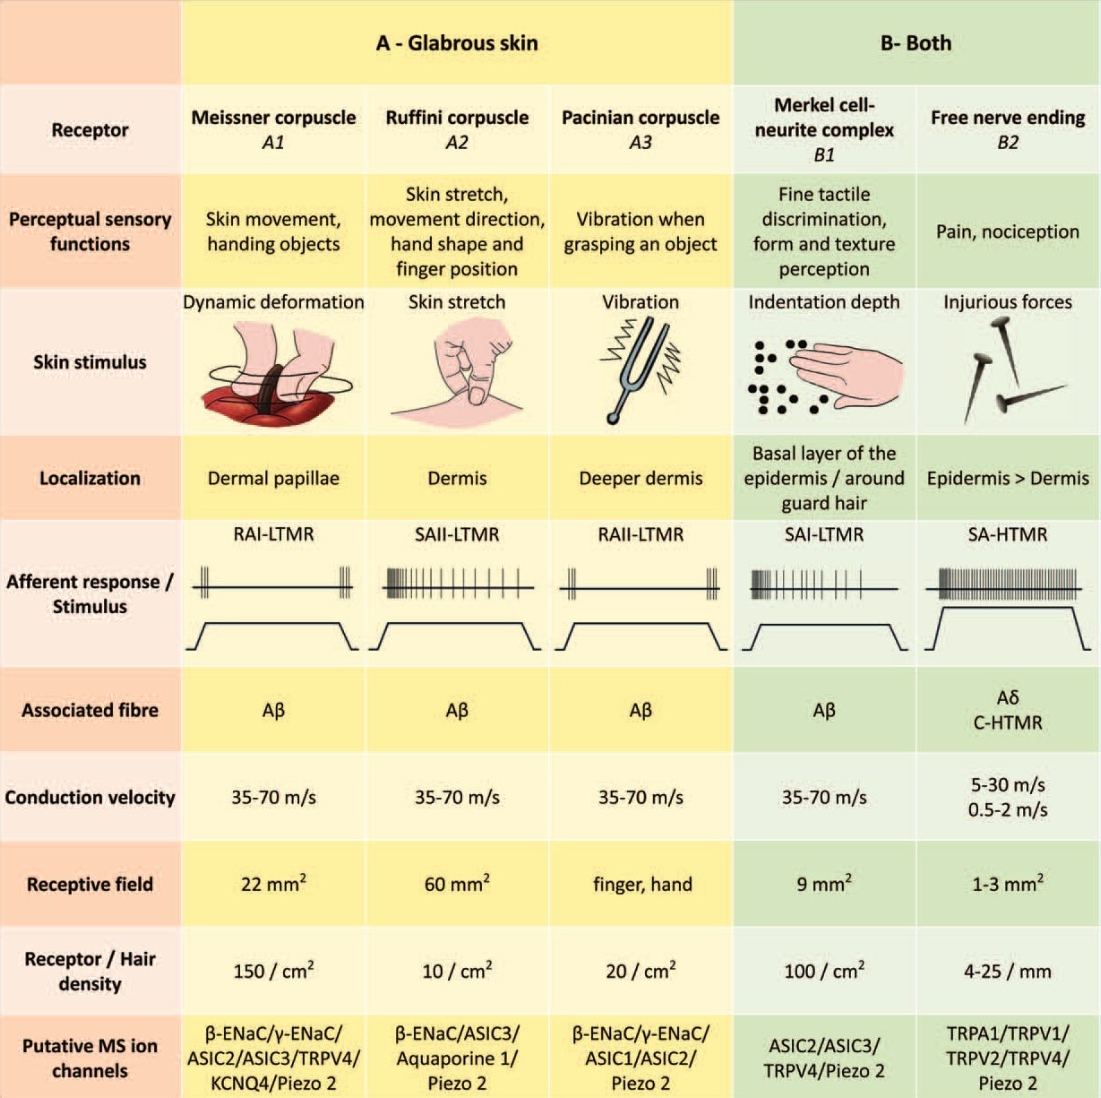
\includegraphics[width=9cm]{Figures/mechanoreceptors-table-cropped.jpg}
%\end{table}
\begin{table}[H]
    \centering
	\caption{Comparison of typical mammalian mechanoreceptor characteristics \cite{Roudaut2012}.}
	\label{tab:mechanoreceptors-table}
	\begin{tabular}{|p{0.19\linewidth}|p{0.21\linewidth}|p{0.21\linewidth}|p{0.21\linewidth}|} \hline
		\textbf{Receptor} & Meissner corpuscle A1 & Ruffini Corpuscle A2 & Pancian Corpuscle B1 \\ \hline
		\textbf{Perceptual   sensory functions} & Skin movement, handling objects & Skin stretch, movement direction,   hand shape, and finger position & Fine tactile discrimination, form   and texture perception \\ \hline
		\textbf{Skin stimulus} & Dynamic deformation & Skin stretch & Indentation depth \\ \hline
		\textbf{Localisation} & Dermal papillae & Dermis & Basal layer of epidermis / around   guard hair \\ \hline
		\textbf{Conduction velocity} & 35 - 70 m/s & 35 - 70 m/s & 35 - 70 m/s  \\ \hline
		\textbf{Receptive field} & 22 mm$^2$ & 60 mm$^2$ & 9 mm$^2$ \\ \hline
		\textbf{Receptor density} & 150 / cm$^2$ & 10 / cm$^2$ & 100 / cm$^2$ \\ \hline
	\end{tabular}
\end{table}
%% Todo: Get copyright permission from image owners


\subsection{Characterising skin}
\label{subsec:Characterising skin}
The sensing qualities of skin is crucial for the sensory feedback in complex manipulation tasks. To aid the creations of technology that mimics qualities of biological pressure sensitive skin, the mechanical properties of must be characterised. Biological human skin is highly variable in terms of its mechanical and sensing properties depending on the region of skin, giving large variation in skin characteristics. Skin can be characterised in terms of the following mechanical characteristics:
\begin{enumerate}
    \item Elastic modulus -  The static elastic properties determined by a linear region of stress and strain of the material. [Pa]
    \item Storage and loss modulus - The dynamic elastic and viscoelastic properties determining the relationship between stress and strain. [Pa]
    \item Ultimate tensile stress (UTS) - The maximum tensile stress that a material can tolerate before breaking [Pa]
    \item Life cycle - The time or number of actuation cycles in which it takes for the actuator to degrade such that it cannot perform its intended purpose to specified standards.
    \item Viscoelastic creep and relaxation - All viscoelastic materials will experience strain creep and stress relaxation to varying degrees depending on the viscoelastic properties of the material. [mm.s$^{-1}$ and s]
    \item Skin thicknesses - the thickness of all layers of skin the cutaneous epidermis and dermis and thickness of the hypodermis. [mm]
    \item Skin surface area - Biological skin has a large surface area and can also be regionalised to map skin function and sensitivity. [m$^2$]
    \item Isotropy/Anisotropy - The directionality of skin properties, also known as skin tension lines, give a topological map of the maximal stretch (i.e. minimal elastic modulus) direction of regions of skin.
\end{enumerate}
Some of the functional properties in terms of pressure mapping include:
\begin{enumerate}
    \item Spatial resolution and touch acuity - The spatial resolution of biological skin, which is mainly dependent on the innervation, mechanoreceptors density, and thickness of the cutaneous layers of skin \cite{Landry2021,Klein2016,Krotoski1993}.
    \item Static force resolution - This is the detection resolution of static or slow-acting forces acting upon the skin \cite{Krotoski1993}.
    \item Temporal resolution - This is the detection resolution of fast-acting forces acting upon the skin often required for texture recognition \cite{Landry2021,Krotoski1993}.
\end{enumerate}

A quantitative characterisation of mechanical and pressure sensing functional skin properties include:
\begin{enumerate}
    \item Elastic modulus -  varies largely depending on test method, test skin type, and subject. Values found in literature include 83.3 ± 34.9 MPa \cite{Annaidh2012}, 0.1 - 2.4 MPa \cite{Khaothong2010}, and 10.4 - 89.4 kPa \cite{Zheng1999}.
    \item Storage and loss modulus - varies largely depending on test method, test skin type, and subject. Values found in literature range include 141.9 ± 34.8 Pa and 473.9 ± 42.5 Pa at 0.8 Hz \cite{Holt2008}, 473.9 ± 42.5 Pa and 32.3 ± 10.0 Pa at 205 Hz \cite{Parvini2022}.
    \item Ultimate tensile stress - 21.6 ± 8.4 MPa \cite{Annaidh2012}. 28.0 ± 5.7 MPa \cite{Ottenio2015}
    \item Life cycle - Skin cells are constantly growing, dying, and shedding. Skin is always actively remodelling based on external stimuli \cite{McGrath2010}.
    \item Strain creep - The strain creep was found to be 2.7 kPa.s for a 10 Pa step input on a dermis skin sample \cite{Holt2008}.
    \item Skin thicknesses - The thickness of human cutaneous skin ranges from 0.6 to 2.6 mm with an average skin thickness of 2 mm \cite{Landry2021}.
    \item Skin surface area - The average surface area of skin in adult humans is 1.7 $\pm$ 0.1 m$^2$ \cite{Landry2021}.
    \item Isotropy/Anisotropy - The tension lines in skin are determined by collagen fibre orientation and dynamic stretch events \cite{Newell2007,Paul2018}. The elastic modulus of human skin was reported to be 160.8 ± 53.2 MPa parallel to the skin tension lines and 70.6 ± 59.5 MPa perpendicular to the tension lines \cite{Ottenio2015}. The UTS of human skin was reported to be 28.0 ± 5.7 MPa parallel to the tension lines and 15.6 ± 5.2 MPa perpendicular to the tension lines \cite{Ottenio2015}.    
\end{enumerate}

\begin{enumerate}
    \item Spatial resolution and touch acuity - The tactile field area increases with indentation depth for certain mechanoreceptors with a range of 5 - 12.6 mm$^2$ \cite{Deflorio2022}. Two point discrimination is another metric for determining spatial resolution an has been determined as 3.7 ± 0.7 mm \cite{Yokota2020}. The receptive field varies depending on the mechanoreceptors used so has been reported to be between 1 and 60 mm$^2$ as another methods of inferring spatial resolution \cite{Roudaut2012}.
    \item Force resolution - Minimum force detection on various regions of human skin was found to be between 67 - 1007 mg \cite{Ackerley2014}, and various mechanoreceptors 0.73 - 122.6 mN \cite{Strzalkowski2015}.
    \item Temporal resolution - Depending on the mechanoreceptor sensing the force input, a frequencies ranges of 0 to 800 Hz can be perceived by human skin \cite{Deflorio2022}
\end{enumerate}


\subsection{Skin Modelling}
% the point of this section is to show that skin is complex to model mechanically and why. Then we can talk about how our composite compares. 
Developing robust mechanical models for human skin is non-trivial for three main reasons:
\begin{enumerate}
    \item High degree of viscoelasticity
    \item Self-regeneration and healing
    \item Constructed from various types of cells in a laminate structure 
\end{enumerate}
To solve the complexity of modelling such a material a review by Landry et al.\cite{Landry2021} shows that many researchers have applied various non-linear mechanical models including Ogden, Mooney–Rivlin, Neo-Hookean, Yeoh, Humphrey, and Veronda–Westmann. When recreating an artificial muscle it is desirable to minimise the mechanical material model complexity so that the material can be more easily integrated into a control system with known behaviour. Similar modelling techniques can be used to model conductive particle elastomer composites due to the similar hyper-elastic and visco-elastic behaviours observed.

\section{Pressure Mapping Artificial Skin Devices}
% Artificial skin review
% Give the range of technologies available expand upon review given in Pt II EIT sensor paper.
This section outlines some of the main technologies which are flexible and/or soft a comparable softness to human skin tissue and can map force events throughout a surface. A particular focus on electro-active polymer (EAP) based sensing is present due to the potential of miniaturising the technology and the range of miniaturised electronics currently available. EAPs are essentially polymer materials which can be used as transducers which change electrical properties based on a mechanical input, vice versa.


\subsection{Soft Pressure mapping technology}
% Why does this section matter? How does it link to my research goals? What is it adding to the greater research pool? A large part of my research was looking into making an 'artificial skin sensor'. It has been requested by several reviewers of my journal article to look at state of the art devices similar to mine, from 2020 onwards and for variant of EIT sensing especially. 
Pressure mapping devices can be categorised into their various sensing technology, such as resistive, capacitive, inductive, magnetic, optical, and acoustic. Transduction methods have been compared by Tiwana et al.\cite{Tiwana2012}, with recommendations to pursue `capacitive, resistive, piezoelectric, piezoresistive or a combination' of methods to replicate mechanoreceptors in the human skin. However, additional optical and magnetic/inductive methods will also be considered in the following sections.

\subsubsection{Resistive}
Soft resistive pressure mapping has been commonly achieved in the past by using arrays of piezoresistive sensor elements, some of which are shown in Table \ref{tab:non_eit_sensor_compare}. The resistive elements can be made using several different flexible piezoresistive materials, such as conductive particle polymer composites\cite{Sun2020,Lu2014,Spahr2017}, intrinsically conductive polymers\cite{Lu2014,Hazelton2023,Mukherjee2023}, microfluidic metals\cite{Park2010,Jung2015,Kim2019}, hydrogel structures \cite{Yuk2016,Park2022,Chen2023}, and flexible piezoresistive semiconductors\cite{Xu2023,Sim2019}.

\begin{table}[H]
		\centering
		\caption{Comparison of different potential piezo-resistive sensor materials. Ranked 1 to 5, where 1 is desirable and 5 is undesirable. WIP - need to redo properly and find a reference for each box!}
		\label{tab:comparing-piezo-r-materials}
		\vspace{3cm}
		\begin{tabular}{|p{2cm}|p{1cm}|p{1cm}|p{1cm}|p{1cm}|p{1cm}|p{1cm}|p{1cm}|p{1cm}|}
			\multicolumn{1}{l}{\textbf{Material:}} & \multicolumn{1}{c}{\begin{rotate}{60} \hspace{0.1cm}\vspace{-2cm} \textbf{Conductivity} \end{rotate}} & 
			\multicolumn{1}{c}{\begin{rotate}{60} \hspace{0.2cm}\vspace{-2cm} \textbf{Piezo-resistivity} \end{rotate}} & 
			\multicolumn{1}{c}{\begin{rotate}{60} \hspace{0.2cm}\vspace{-2cm} \textbf{Hardness} \end{rotate}} & 
			\multicolumn{1}{c}{\begin{rotate}{60} \hspace{0.2cm}\vspace{-2cm} \textbf{Manufacturability} \end{rotate}} & 
			\multicolumn{1}{c}{\begin{rotate}{60} \hspace{0.2cm}\vspace{-2cm} \textbf{Cost} \end{rotate}} & 
			\multicolumn{1}{c}{\begin{rotate}{60} \hspace{0.2cm}\vspace{-2cm} \textbf{Durability} \end{rotate}} & 
			\multicolumn{1}{c}{\begin{rotate}{60} \hspace{0.2cm}\vspace{-2cm} \textbf{Toxicity} \end{rotate}} & 
			\multicolumn{1}{c}{\begin{rotate}{60} \hspace{0.2cm}\vspace{-2cm} \textbf{Drift} \end{rotate}} \\ \hline
			
			Conducting polymer & 5 & 3 & 3 & 2 & 2 & 3 & 2 & 3 \\ \hline
			Electrolytic hydrogel & 1 & 2 & 4 & 3 & 4 & 2 & 2 & 2   \\ \hline
			Conductive particle polymer & 2 & 4 & 4 & 4 & 4 & 4 & 2 &  \\ \hline
			Conductive particle paste & 3 & 2 & 4 & 3 & 4 & 2 & 3 & 2  \\ \hline
			Conductive textile & 4 & 4 & 3 & 2 & 4 & 5 & 4 & 3  \\ \hline
		\end{tabular}
\end{table}

\subsubsection{Capacitive}
Similar to resistive pressure mapping, capacitive pressure mapping has more commonly been done using arrays of capacitive elements. Many capacitive touch sensors use the human body to shunt the electric field between the capacitor electrode(s) to a common ground. However, the operating principle of capacitive-based strain sensors rely on the deformation of the capacitor dielectric and/or the capacitor electrodes \cite{Sapra,Zhu2021,Liang2015}
\begin{figure}[H]
	\centering
	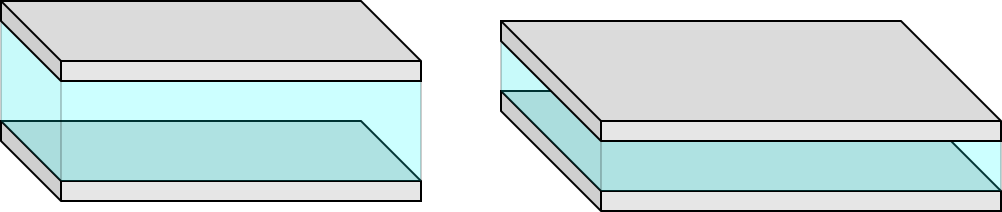
\includegraphics[width=0.6\linewidth]{Figures/cap_deformed_states_x2_crop.png}
	\caption{Two grey electrodes across a blue dielectric medium. Left: Uncompressed state. Right: Compressed state exhibiting larger electrode areas and a thinner dielectric thickness.}
	\label{fig:cap_deformed_cube}
\end{figure}

\subsubsection{Magnetic}
Magnetic strain mapping devices can be achieved using several methods. One method is to have a three layer stack with hall effect sensors \cite{Yan2021}. The stack is made up of a the bottom layer full of rigidly connected three dimensional hall effect sensors, the second layer is made from an elastomer, and the top layer has a magnetic particle unit placed at a set distance above each of the hall effect sensors. The movement of the magnets alters the magnitude and direction of magnetic field sensed and data can be interpolated to create a map of strain deformation. The main advantages of this method is that each hall sensor can detect in three dimensions, hence normal and shear forces can be detected, and using magnetismfor sensing means less electrical noise in the system. The main disadvantages of this method of sensing is the added complexity in scaling the system and the electronics required and the rigid surface required.  

\subsubsection{Optical}
There are various methods for making a optically driven artificial skins. A recent review has been curated by Lee et al. \cite{Lee2023} all of the different methods of using optics for creating tactile sensors. The main advantages of optical sensors include the high speed sensor response, immunity to electrical noise, and their non-invasive nature. The main disadvantages include, the bulky hardware required for driving the optics and signal processing, the potential interference of external light sources, and the materials that can carry optical signals. 

\subsubsection{Acoustic}
Acoustic soft tactile sensing has not been explored much compared to the other forms of sensing given. Park et al., Hughes and Correll \cite{Park2022,Hughes2015} have created a system which uses passive acoustic tomogrpahy (PAT) to localise and and classify different types of touch. This form of tactile sensing is the most similar to the biological system of mechanoreceptors which are specialised to detect certain frequencies of vibration.

%%% COMPARISON OF NON-EIT SENSOR EQUIVS %%%
%\newpage
%\newgeometry{left=0.5cm,right=0.5cm,bottom=0.5cm,top=0.5cm}
%\afterpage{%
%	\clearpage% Flush earlier floats (otherwise order might not be correct)
%	\thispagestyle{empty}% empty page style (?)
%	\begin{landscape}% Landscape page

\subsubsection{Soft Pressure mapping technology comparison}
The softness of biological human skin has a large range as discussed in Section \ref{subsec:Characterising skin}. There have been a range of works investigating sensors with a range of softness' and performance. A comparison of these start-of-the-art soft sensor works is given in Table \ref{tab:non_eit_sensor_compare}.
%%% COMPARISON OF NON-EIT SENSOR EQUIVS %%%
%\newgeometry{left=2in,right=0in,bottom=0in,top=2in}
\begin{landscape}
		\newcolumntype{L}[1]{>{\raggedright\let\newline\\\arraybackslash\hspace{0pt}}m{#1}}
		\thispagestyle{plain}
		 \begin{table}[H]
		 	\caption{Comparison of soft sensor technologies.}
		 	\label{tab:non_eit_sensor_compare}
			\begin{tabular}{|L{2.9cm}|L{2cm}|L{2.5cm}|L{3cm}|L{2.9cm}|L{2cm}|L{3cm}|L{2cm}|L{2cm}|} \hline 
				\textbf{1st Author} & \textbf{Sensing principle} & \textbf{Sensing region material} & \textbf{Sensing region elastic modulus or shore hardness} & \textbf{Electrodes per sensing position} & \textbf{Repeatability} & \textbf{Time series data shown} & \textbf{Spatial resolution} & \textbf{Temporal resolution} \\ \hline
				Gilanizadehdizaj \citep{Gilanizadehdizaj2022} & Piezo-resistive & Ecoflex30-00 rGO composite sponge & 40 kPa & 2 sensels / electrode & 10 cycles for each stress & \textit{-} & 10 x 10 mm & - \\ \hline
				Fu\citep{Fu2020} & Piezo-resistive & Carbon black silicone composite & 1.5 Mpa & 0.625 sensels / electrode & 50000 cycles & Yes. & 12 x 12 mm & 60 ms \\ \hline
				Yang\citep{Yang2022} & Piezo-resistive & Ecoflex graphene composite sponge & - & 2 sensels / electrode & 800 cycles & Yes. & 10 x 10 mm & 150 ms \\ \hline
				Liang\citep{Liang2015} & Capacitive & PDMS, PET, Si, Sio2, Cu laminate & 4000 Mpa & 1 sensel / electrode & - & Real-time use of sensor shown. No explicit time-series data. & 4 x 4 mm & - \\ \hline
				Yan\citep{Yan2021} & Magnetic & Ecoflex 00-50 & 83 kPa & 11 IC pins / sensel & 30,000 cycles & Yes. & 0.1 x 0.1 mm & 15 ms \\ \hline
				Rossiter\citep{Rossiter2005} & Optical & Polymer foam & - & 2 sensels / electrode & - & - & 10 x 10 mm & - \\ \hline
				Shimdera\citep{Shimadera2022} & Optical & Super clear silcone & 40 A & N/A. One fiber optic LASER and   one camera. & Error increase of 1.7\% over 30   days & Yes. & approx. 20 x 20 mm / 0 - 1100 um & Sample rate 1.6s. Training   required. \\ \hline
				Ramuz\citep{Ramuz2012} & Optical & PDMS & - & N/A. Two arrays of OLEDs and   Organic Photo Detectors used. & 900 cycles & Yes. & Not localised. & 300 ms \\ \hline
			\end{tabular}
		\end{table}
\end{landscape}
%\captionof{table}{All `-' values are not present in the paper reviewed}% Add 'table' caption
%\end{landscape}
%\clearpage% Flush page
%}


%% LEAVE THIS LIT REVIEW AS BACKGROUND IN THE RELEVANT CHAPTERS??
% \subsection{Electrical Impedance Tomography}
%% % How does EIT work
%
% \subsection{Electric Field Imaging}
% % Quick review on the theoyr of EFT and how it differs from EIT. Discuss it's importance and reference how this work looks towards using capacitive shunting AND EIT to create a faster EIT-based pressure mapping sensor.
%
% \subsection{EIT-based Skins}
%% % Give a review on the state of art EIT-based skin technology


\section{Biological Muscle form and function}
% lit review on 'An engineering perspective on the function of human muscle'
%\textit{Note: This section was taken from literature reviews from 3 years ago, when I was going to research DEAs. Needs a re-review ASAP.}

Biological muscles are a product of millions of years of evolution and the motion and other mechanical characteristics of biological structures is yet to be outperformed by artificial muscle technology. To determine how to quantify the performance of a biological muscle this section gives foundational knowledge about muscle function, structure, and how it can be characterised from an engineering perspective rather than the typical biological perspective, so that similar actuator devices with similar attributes can then be investigated.

Biological muscle is a naturally occurring tissue comprised of muscle fibres bundled together to apply a contractile force on connecting tissue or, in the case of smooth muscle, applying a force on itself. The base actuator units of muscle are proteins myosin and actin filaments, which effectively slide against each other to produce a contractile motion. The root cause of a muscle contraction is an electrochemical signal sent from the central nervous system to a motor neuron/s which travel to the muscle where electrochemical reactions take place for the contraction to occur\cite{Keynes2011}.
\begin{figure}[h!]
	\centering
	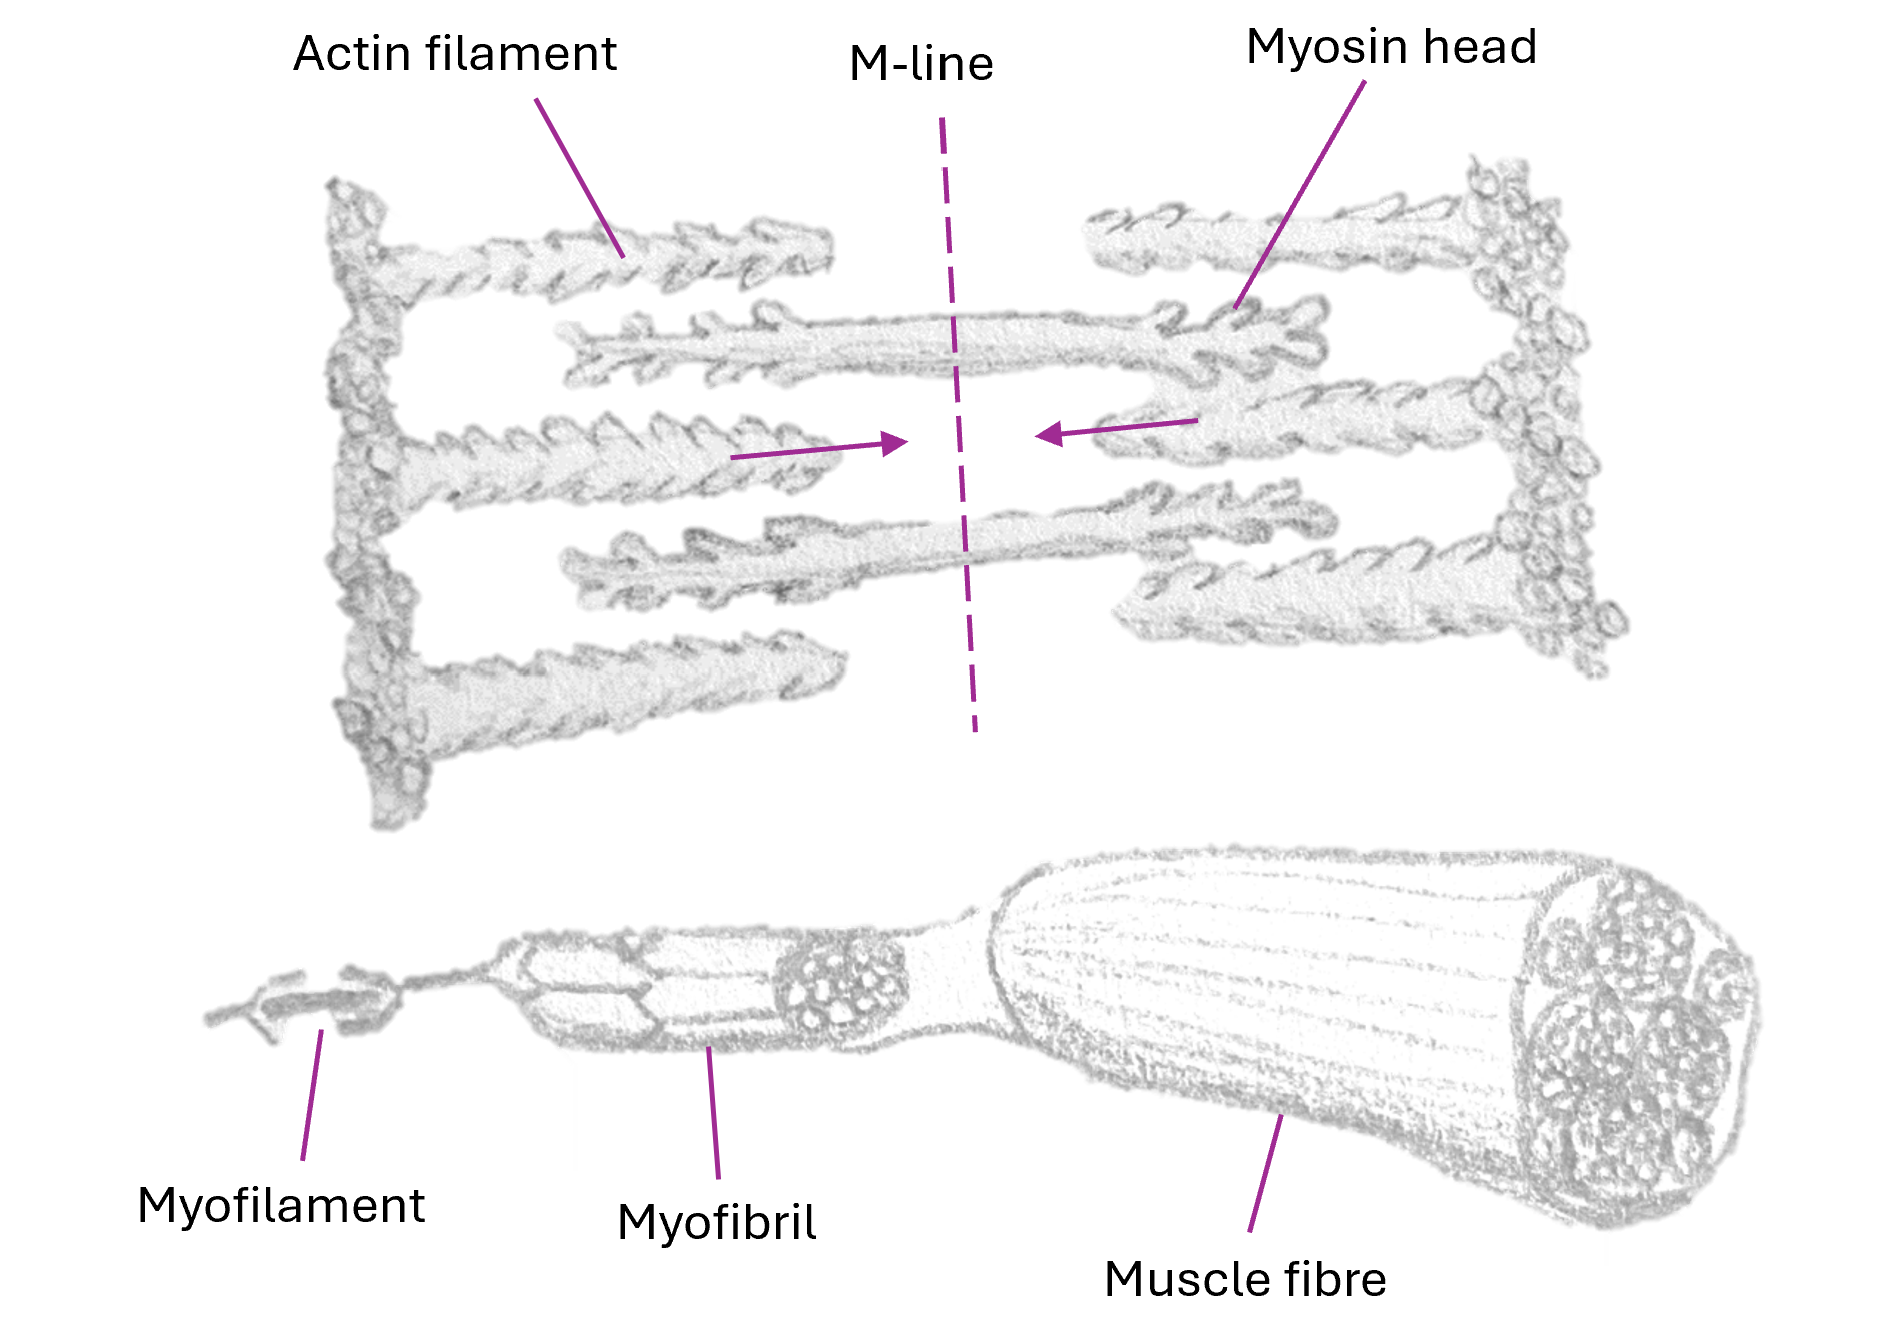
\includegraphics[width=0.6\linewidth]{Figures/motor-unit-myo-fibril-to-fibre.png}
	\caption{Components of a biological muscle contractile unit and meta-structure.}
	\label{fig:muscle_units}
\end{figure}
The sliding motion of the myosin and actin filaments is due myosin heads binding to the actin and pulling the actin towards a middle line (M-line) in multiple stroke actions. These filament actuators are stacked in three dimensions within a muscle fibre to amplify contractile stress and strain as shown in Figure \ref{fig:muscle_units}.

On a macro scale, muscle is made up of bundles of fasicles connected together with a tissue called perimysium. Within the fasicles are many muscle fibres (i.e. muscle cells) which are surrounded by a connective tissue called endomysium. Within the muscle fibres there are many sacromeres stacked within a cyclindrical-like structure called a myofibril. Each sacromere contains a contractile unit of myofilaments. 



\subsection{Characterising a muscle}
To quantify the performance of a biological muscle, certain metrics are compared. An artificial and biological muscle can be characterised using typical mechanical material parameters such as:
\begin{enumerate}
    \item Stress - Force that is applied to the normal of the cross section of the muscle through various states of muscle excitation. [$Pa$]
    \item Strain - The muscle change of length due to the stress applied through various states of muscle excitation. [\%]
    \item Elastic modulus - The elasticity determining the relationship between stress and strain for the linear region of the stress strain characteristic curve. [$Pa$]
    \item Energy density - The work done by the muscle per unit volume or mass. [$J.kg^{-1}$]
    \item Power density - The work done by the muscle per unit volume or mass per unit time. [$W.kg^{-1}$]
    \item Ultimate tensile strength - The maximum tensile stress that a material can tolerate before breaking. [$Pa$]
    \item Efficiency - The work done by the muscle compared to the energy put into the system, known as metabolic cost in biological muscles. [\%]
    \item Actuation frequency - The frequency range of actuation cycles using the system's method of excitation. [$Hz$]
    \item Stroke - The maximum displacement an actuator can achieve [$m$]
    \item Life cycle - The time or number of actuation cycles in which it takes for the actuator to degrade such that it cannot perform its intended purpose to specified standards.
\newline
\newline
    As well as the commonly used medical/biological muscle metric:
\newline
    \item Maximum isometric contraction force - the maximum force a muscle can apply without changing strain. This is also related to the ratchet-like mechanism and muscle locking where a muscle can apply a much larger force in a static state, as seen in the myosin binding\citep{Cross2006}.

\end{enumerate}
Other qualities of muscle should be quantified on a case by case basis depending on the artificial muscle technology being investigated. For example, a major issue with dielectric elastomer actuators is the excitation voltage required for actuation is too large for many applications. Hence, excitation voltage could be another parameter considered for some electroactive artificial muscles.

Some of the biological muscle metrics have been quantified by previous research as seen below:
\begin{itemize}
    \item Energy density - energy densities ranging from 0.4 - 40 $J.kg^{-1}$\citep{Alexander1977}.
    \item Power density - power densities ranging from 9 - 284$W.kg^{-1}$\citep{Full2004}
    \item Actuation frequency - natural actuation frequencies ranges 1 to 180$Hz$\citep{Full2004}.
    \item Strain - ranging from 5 - 30\%\citep{Duduta2019}.
    \item Efficiency - Thermodynamic efficiency of human muscle is typically between 20-35\%\citep{Smith2005}. However other biological muscle has been seen to reach efficiencies of up to 77\%\citep{Smith2005}.
\end{itemize}
    

\subsection{Muscle Mechanics}
Before attempting to recreate a bio-mimetic actuator it is important to acknowledge the numerous simplified electro-mechanical system models of parts of the muscle actuation process. These models need to be understood to gain an understanding of the application of biomimetic actuators can be used in assistive soft robotic devices. From here we will present basics of the subject of bio-mechanics.

The stress and strain involved in muscle contraction is more complex than uniform materials and is non-linear. The stress and strain of a passive muscle (i.e. contractile units are not producing internal muscle tension) can be modelled with the following equation; 
\begin{equation}
    \frac{d\sigma}{d\varepsilon} =  \alpha.(\sigma+\beta)
\end{equation}
Where $\varepsilon$ \& $\sigma$ are strain and stress respectively. A solution for this is first order ODE is; 
\begin{equation}
    \sigma = \mu e^{\alpha\varepsilon} - \beta
\end{equation}
Where $\mu$ is a free parameter determined empirically. The stress-strain of a passive muscle can be likened to tension being applied yarn. As more strands of the yarn are pulled into tension the stress increases, then as the last strands are brought into tension a maximum stress is reached, until the yield stress is reached. Linear approximations can still be made over regions of elongation depending on accuracy required for application. The stress-strain of an active muscle (i.e. when it is tetanised) is approximated to a piece-wise quadratic function or bell curve. It is important to note that the stress for both active and passive muscle is zero when the strain is less than 0.4, demonstrating the yarn-like nature of the muscle stress-strain as shown in Figure \ref{fig:muscle-fibre-stress}.
\begin{figure}[H]
  \centering
  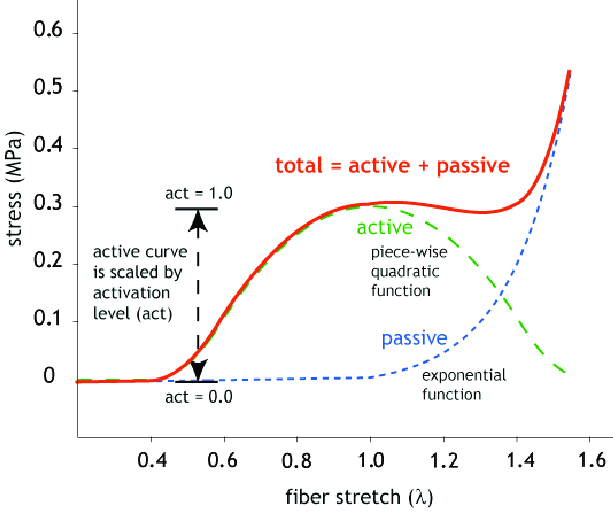
\includegraphics[width=8cm]{Figures/Muscle-fiber-active-and-passive-behavior.png}
  \caption{Stress and strain of active and passive muscles ($\copyright$ J. Teran $|$ ACM 2003)\citep{Teran2003}}
  \label{fig:muscle-fibre-stress}
\end{figure}
Hill's muscle models commonly refer to a mechanical three element model \citep{Hill1938} composed from, one parallel non-linear spring element, one series non-linear spring element, and a contractile unit.
%\begin{figure}[H]
%  \centering
%  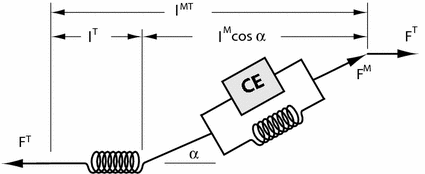
\includegraphics[width=8cm]{Figures/hill_type_muscle_model.png}
%  \caption{Hill muscle model\citep{Arnold2010}}
%  \label{fig:hill-model-Muscle}
%\end{figure}
%Where $F^{KT}$ and $F^{KM}$ are the spring forces of the tendon and muscle respectively, which are a function of extension length. $F^CE$ is the contractile force and $F^T$ is the total contractile force as observed at the end of each tendon either end of the muscle. Where  $F^T$ is the tendon force; $F^M$ is the muscle force; the $l^T$, $l^M$, $l^{MT}$ are muscle length, tendon length and their combined lengths respectively; $\alpha$ is the pennation angle (i.e. zero if parallel muscle); The left and right non-linear spring elements represent a tendon and muscle spring characteristic respectively; The CE box represents the contractile element that generates contractile force. 
%\begin{equation}
%    F^T = F^{KT} + (F^{CE} + F^{KM})cos(\alpha)
%    \label{eqn:hills-model}
%\end{equation}


\subsection{Electrical Muscle Models}
Similar to EAP-based artificial skin and artificial muscles, biological muscles also require electrical stimulation to function. The main method for providing an artificial electrical stimulation to a muscle, to simulate the signal a motor neuron would give to a muscle, is functional electrical stimulation (FES). Due to the biochemical nature of the motor neuron signal transport and the purely electrical stimulation provided by the FES device, the process isn't as efficient as the naturally occurring electro-chemical muscle activation, often resulting in increased muscle fatigue when compared to equivalent voluntary muscle contractions \citep{Ibitoye2016}. FES applies a voltage across between two electrodes on the user's skin above a specific muscle. The voltage simulates the signal form and frequency of action potentials between 4 - 12Hz\citep{Popovic2004}. The threshold for a muscle action potential to cause a muscle contraction is approximately 70 mV \cite{Schmidt-Nielsen2002}.
%\begin{figure}[h!]
%  \centering
%  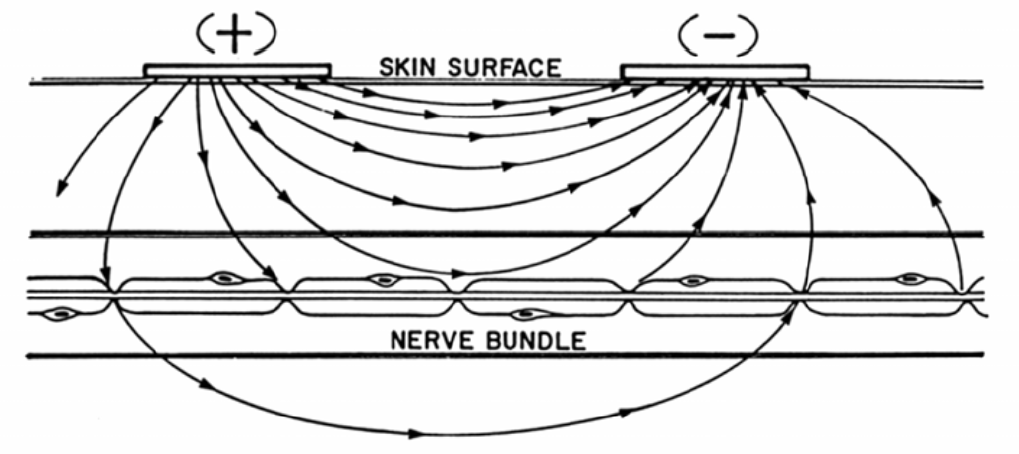
\includegraphics[width=8cm]{Figures/FES_electric_field.PNG}
%  \caption{Electric field generated by two electrodes on the surface of the skin above a specific muscle and hence it's activating nerve bundle\citep{Bajd2010}}
%  \label{fig:Muscle}
%\end{figure}
To artificially sense an intended muscle contraction electromyography (EMG) can be used. EMG also commonly uses two electrodes on the surface of the skin above a desired muscle. This EMG signal can be used as a sensor input for joint pose estimation. EMG senses the action potential impulses conducted along motor neurons to the muscle. 
There are many models for limb motion and EMG- and FES-based therapies \cite{Meadmore2014,Freeman2015,Hodkin2018,Popovic2014}.




\section{Artificial Muscle Technology}
There are many types of electrically actuated artificial muscles technology. Artificial muscle actuator technology that has gained particular interest in recent years include, the ionic polymer-metal composite (IPMC) actuator, the hydraulically amplified self‐healing electrostatic (HASEL) actuator, magnetorheolgical elastomer (MRE) actuators, and dielectric elastomer actuators (DEAs). Each of these having qualities very similar to that of biological muscle usually with a trade-off in actuation response time, actuation force, and actuation strain for their various possible topologies. This section gives a brief overview of four state-of-art soft electromagnetically driven actuator technologies.

\subsubsection{Ionic polymer–metal composite actuator}
Ionic polymer-metal composite actuators (IPMCs) are soft actuators that can be actuated at a much lower excitation voltage than DEAs, commonly less than 10V. IPMCs are also desirable as artificial muscles they have shown large bending deformations, simple to fabricate, light weight and thin in design, and can have a fast actuation response time ($>$15Hz) at small displacements\citep{Ma2020}. IPMCs also have a high work density and maintain a constant volume during actuation like biological muscles\cite{Neuhaus2020}.
\begin{figure}[h!]
  \centering
  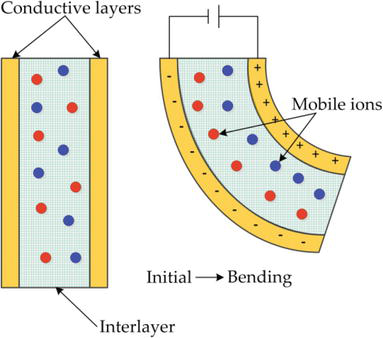
\includegraphics[width=0.5\linewidth]{Figures/IPMC.png}
  \caption{Diagram of the typical architecture of an IPMC actuator\citep{Yanjie2018} ($\copyright$ 2018 Yanjie Wang and Takushi Sugino)}
  \label{fig:Artificial Muscle_IPMC}
\end{figure}
An IPMC is made up of an ionic polymer interlayer, two electrode conductive layers, and a voltage source. The ionic polymer interlayer allows for ionic transport and is typically made of treated Nafion or Flemion. These materials are typically used as ion exchange membranes so have the characteristics desired for the transporting ions during the actuation of the IPMC actuator. The two electrodes are made of a suitably conductive and flexible material. The interlayer is treated such that it is filled with water molecules and cations, with the chemical backbone of the interlayer being slightly negatively charged. When a voltage is applied across the electrodes the cations are repelled from the cathode and travel towards the anode while the water molecules are displaced in the opposite direction towards the cathode. The ionic polymer then swells as the cations repel each other along the anode side of the interlayer, while the polymer elements on the cathode side effectively shrink\citep{Segalman1999}. This swelling adjacent to the cathode provides the device's bending actuation.

There are many variations of the design and manufacturing of IPMCs to optimise the actuator for an application as shown by \cite{Shahinpoor2016}.Although the process of manufacturing IPMCs is simple, it takes a long amount of time (often $>$48 hours\citep{Ma2020}) for the ionic polymer interlayer to absorb the necessary ions and undergo the necessary reactions. There has been much research into the optimal manufacturing of an IPMC \citep{HOMMA1999,Liu1992,Shahinpoor2016}. The use of additive manufacturing has been used successfully to generate more complex geometries using fused filament deposition\citep{Carrico2015}.

IPMCs can also be used as sensors. When an IPMC undergoes bending due to an external force there is a potential generated across the electrodes, which indicates bending direction and magnitude\citep{Shahinpoor2004}.

Two key deficiencies of current IPMC actuator technology are the maximum force output achievable and the life cycle of the actuator in a dry (non-aqueous) environment.The force output optimisation of IPMCs has been investigated by several researchers, all of which having a maximum actuation force in the milli-newton scale \citep{Akle2004,Xu2014,Shahinpoor2004}. 
Because the IPMC actuators rely on hydrated ionic transport to actuate this means if the IPMCs are in a dry environment then over time they will decrease their maximum actuation force.

The applications of this actuator is limited to applications requiring a small actuation force and a wet environment. Current applications include flexible catheters \citep{Guo1994}, small biomimetic robotics \citep{Kodaira2019,Chang2013}, aquatic robotics\citep{Hubbard2014,Khawwaf2019}, with many other applications yet to be discovered.

\subsubsection{HASEL actuator}
A hydraulically amplified self‐healing electrostatic (HASEL) actuator is a recent soft actuator technology developed in 2018\citep{Kellaris2018} which displays many qualities that are better than current artificial muscle technology. HASEL actuators are made up of three main components: electrodes, dielectric fluid, and an elastomeric shell. The electrodes need to be highly conductive, able to handle high electric potential, and can be solid or flexible. Hydrogel electrodes have been proven to be a good material for the electrodes because of their elasticity while still maintaining a high conductivity\citep{Acome2018}. In one application the hydrogel material is bonded to a polydimethylsiloxane (PDMS) substrate for mechanical strength and for ease of bonding to the actuator biaxially-oriented polypropylene (BOPP) shell\citep{Kellaris2018,Yuk2016}. HASEL actuators use high electric potential across two electrodes to create an electrostatic force. This force induces a zipping effect which pulls the electrode together from one end to the other as the electric field strength increases. The zipping of the two electrodes pushes the dielectric fluid into the reservoir increasing the pressure which alters the shape of the reservoir bounds providing an actuation motion. When the electrodes have displaced all of the fluid between them the actuation displacement is at a maximum. The electrostatic zipping action allows a large force to be generated due to snap-through transition. Snap-through transition is an actuation instability which has been discussed in previous research as a means of amplifying DEA actuation strain\citep{Keplinger2012}. 
\begin{figure}[h!]
  \centering
  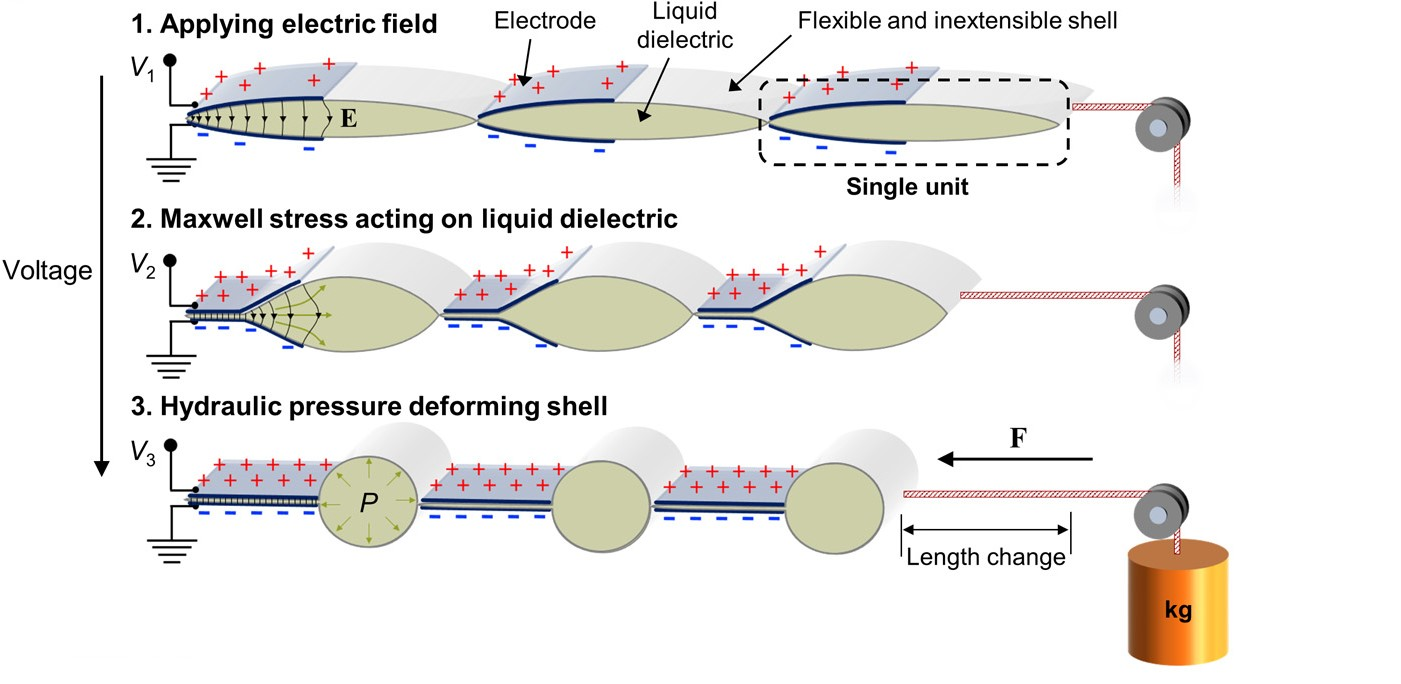
\includegraphics[width=0.7\linewidth]{Figures/HASEL_actuator_crop.jpg}
  \caption{Diagram of the typical architecture and the contraction stages of a HASEL actuator\citep{Kellaris2018}}
  \label{fig:Artificial Muscle_HASEL}
\end{figure}
Recorded efficiency values of HASEL actuators of 21\% are comparable to that of human muscles of 20 - 35\% \citep{Smith2005}. The actuators have had a frequency response of up to 20Hz. Large strains of 124\% have been recorded, but can only be achieved when actuating at a resonant frequency. Strains of up to 79\% have been recorded using a linear planar HASEL actuator configuration and DC voltage stepping.  Else, strains of only 10\% have been recorded for static steady strain\citep{Kellaris2018}.
Because there is a relationship between the motion of the actuation and capacitance between the electrodes, this means self sensing can be achieved through the electrodes. Although due to the flexible and fluid nature of the device, modelling of the HASEL is difficult and limited in accuracy.

The simple and commonly used manufacturing process for HASEL actuators is completed in six steps as shown by the diagram below:
\begin{figure}[h!]
  \centering
  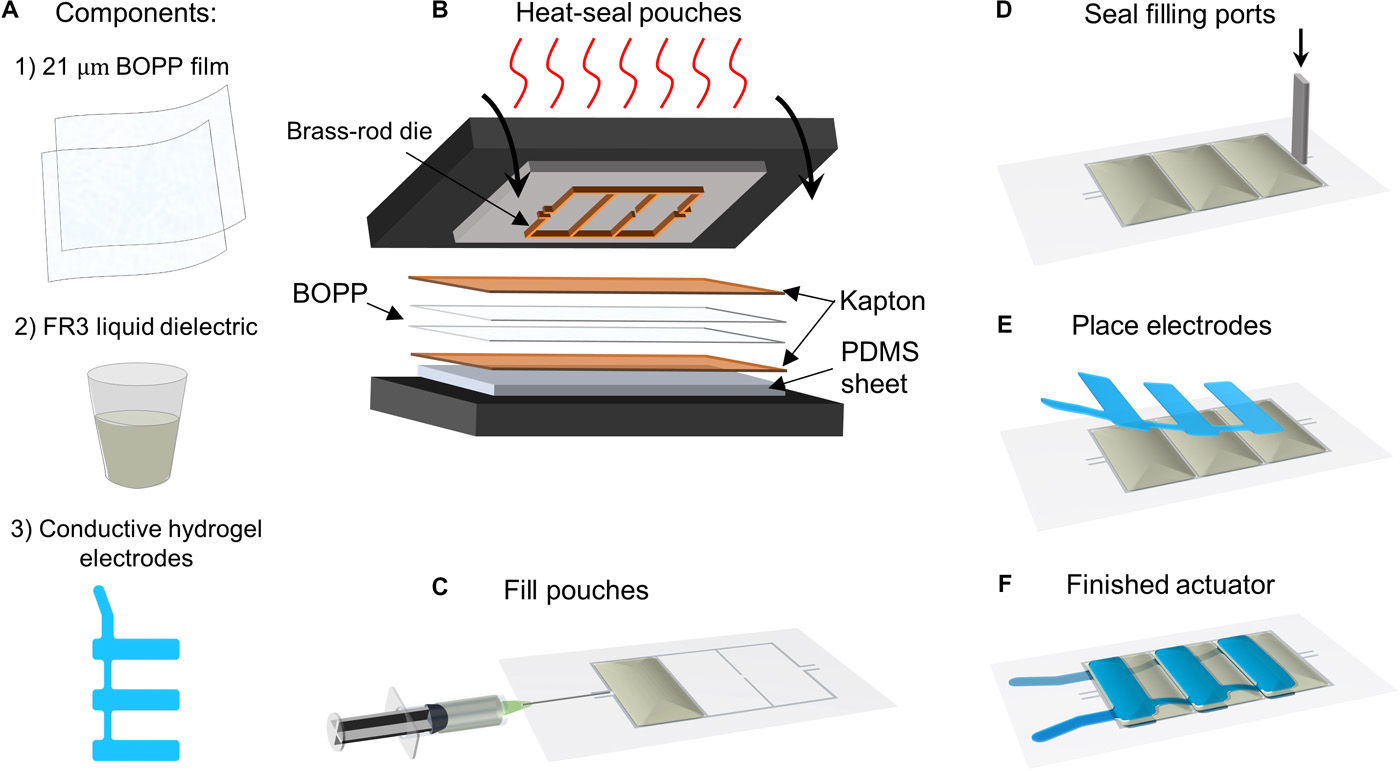
\includegraphics[width=0.7\linewidth]{Figures/HASEL_manuf.jpg}
  \caption{Diagram of the simplified stages of HASEL actuator production\citep{Kellaris2018}}
  \label{fig:Artificial Muscle_HASEL_manf}
\end{figure}

Other attempts have been made to use polyjet inkjet based additive manufacturing to make the whole HASEL actuator and have been successful with proof of concept, but are yet to be developed from prototype stage\citep{Manionn.d.}. 

The cyclic life of HASEL actuators are high, because of their self-healing properties. When there is a dielectric breakdown through the liquid dielectric the damage caused is not permanent like when a DE breaks down. The liquid may form some small air bubbles, however these may not effect the operation of the actuator, instead this can increase the likelihood of a another dielectric breakdown. The cycle life of the HASEL actuator was seen to be larger than one million with a given torus shaped HASEL actuator\citep{Acome2018}. The HASEL technology is promising with a number topologies possible, some topologies include toroidal, planar linear\citep{Acome2018}, and scorpion metasoma(tail)\citep{Mitchell2019}.

\subsubsection{Dielectric Elastomer Actuators}
% How do DEAs work
The dielectric elastomer actuator (DEAs) are often called artificial muscles because they share similar characteristics to biological muscle such as, the large strains achievable, the high elastic energy density, many topologies/configurations achievable, and constant volume during its contraction.

A DEA consists of a dielectric elastomer (DE) film sandwiched between two compliant electrodes. To excite the actuation, a high electric potential is applied to across the electrodes creating an electrostatic force between the two compliant electrodes. This force pulls the two electrodes together applying stress (known as Maxwell's stress) to the elastomer and hence strain parallel and perpendicular to direction of the electrostatic force. When the DEA is contracted the surface area of the electrodes increases and the thickness of the DE decreases causing a change in capacitance and Maxwell's stress.
\begin{figure}[h!]
	\centering
	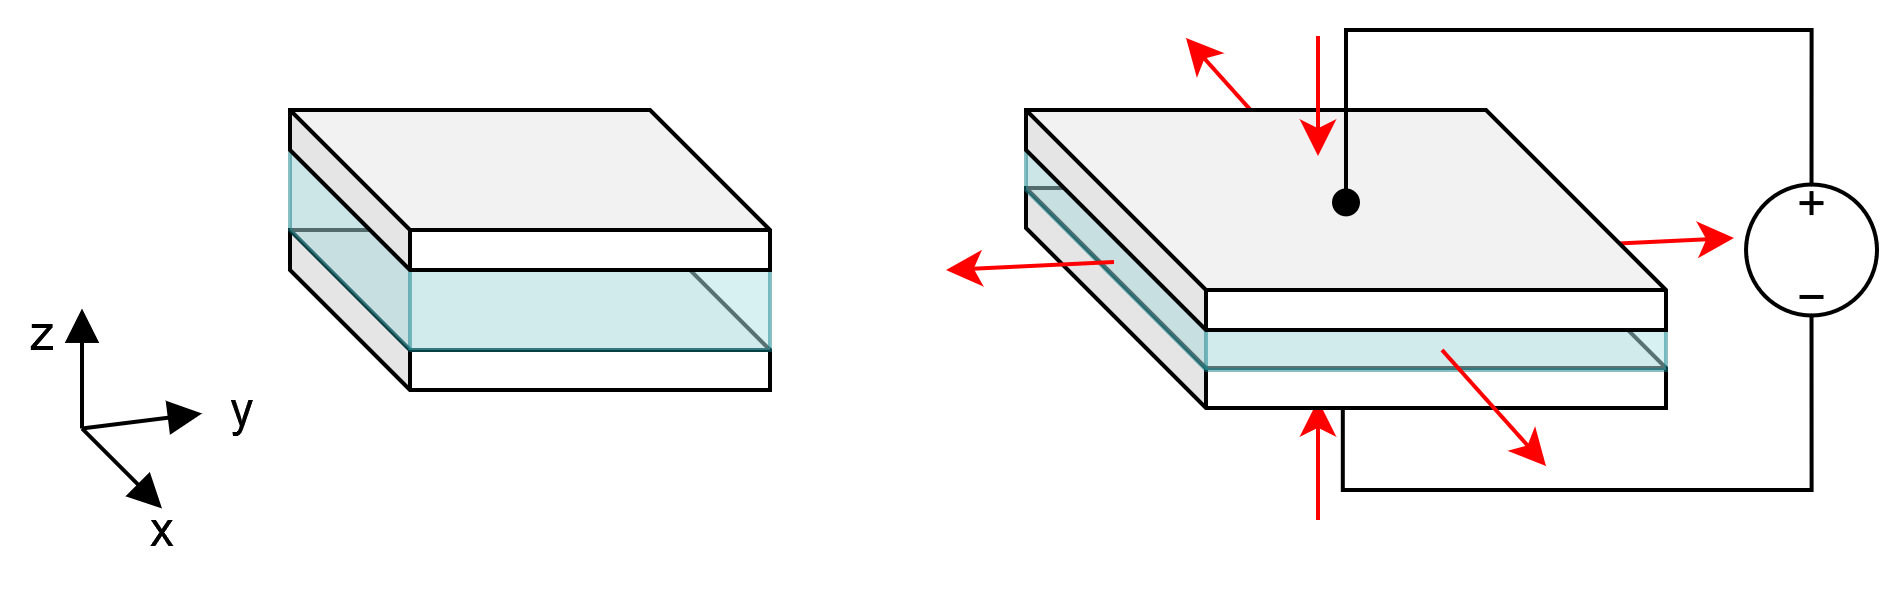
\includegraphics[width=0.7\linewidth]{Figures/dea_square_2state.jpg}
	\caption{DEA with two compliant light-grey electrodes and a transparent light blue dielectric elastomer. Showing deformation without and with a voltage applied across the electrodes.}
	\label{fig:Artificial Muscle_DEA}
\end{figure}
A dielectric elastomer actuator can be modelled as a flexible parallel plate capacitor in its simplest form. Using this we can determine the electrostatic pressure to be:
\begin{equation}
	\sigma_{es} = \varepsilon_0 \varepsilon_r \frac{V^2}{z^2}
\end{equation}
Where $\sigma_{es}$ is the electrostatic pressure, $\varepsilon_0$ and $\varepsilon_r$ are the vacuum and relative permittivity constants, $V$ is the voltage potential applied across the electrodes and $z$ is the thickness of the DE. The electrodes used for a DEA need to be made of a conductive material, but require similar elasticity to the dielectric material. An ideal material for these electrodes would have high conductivity. This conductivity would change minimally and predicatively under large strains. Many composites have been used in practice for these electrodes, with the most common in early development being a silicone rubber and carbon powder composite. However, the unpredictable nature of carbon powder elastomer composites has lead to research into many other materials/silicone additives such as hydrogels, graphene sheets, metallic nanostructures, carbon nanotubes, liquid metal\citep{Liu2013,Rogers2013,Bele2018,Quinsaat2015}. The ideal material for the dielectric elastomer should have a high elastic modulus and a high electric breakdown voltage. The elastic modulus needs to be sufficiently high so that less electrostatic pressure can create a larger strain. While the breakdown voltage of the material needs to be sufficiently high such that the material will not break down at the maximum desired strain. If a material can be found with a high enough electric breakdown strength at a smaller thickness than current research prototypes then a higher stress can be achieved giving a larger or equivalent actuation force at a lower voltage.

Many other topologies exist to generate different actuation motions using the same electrostatic pressure generation principle. These include actuator topologies such as stack\citep{Hau2018,Kovacs2009}, helical\citep{Carpi2012}, bending\citep{Pfeil2020}, lens\citep{Ghilardi2019}, cylindrical, and rolled shaped actuators\citep{Amin2018}. Each of which having a range of applications.

DEAs are often fabricated in a laboratory environment using a pre-strained elastomer. The pre-straining accomplishes four key qualities; stores elastic strain energy, ensures DE is planar within the bounds of the jig, controls the initial thickness of the DE, and puts the DE in an optimal stress-strain region, often taking advantage of elastomer hyper-elasticity. There is no standard practice for the fabrication of DEAs, other methods such as additive manufacturing have also been explored to generate more complex geometries and to increase production speed\citep{Park2018,McCoul2017}.

As well as actuating, DEAs can also be used for sensing. DEAs can be used as sensitive capactive sensors, where any strain applied to the DE will relate to the effective capacitance between the two electrodes\citep{Jung2008,Goulbourne2007,Gisby2013}. 

Currently dielectric elastomer actuators all require voltages within the kilo-volt range to generate an adequate stress and strain for a range of applications. A key problem encountered by researchers designing DEAs is the trade-off between actuation force and strain magnitude \citep{Hau2018}. This high voltage requirement may deem the technology dangerous for use where there is a possibility that a human may come into physical contact with the high voltage electrodes.
% Give a review on state of art DEA technology??

\subsubsection{Magnetorheological Elastomer}
Magnetorheological elastomer (MRE) actuators, also known as magnetoactive soft materials (MSMs), are a relatively new form of actuator however the theory reinforcing operating principle has been known since at least the 1980s \citep{Jolly1996}. The structure of an MRE actuator generally consists of a ferromagnetic elastic composite and a driving magnetic field. An example of this is a composite of iron-carbonyl powder and PDMS. The operating principle of MREs is that magnetic flux travelling through the MRE will change mechanical characteristics within the elastomer (i.e. stiffness or displacement of the body). The operation of a MRE actuator is similar to a DEA however instead of having an electric field cause a contraction it is a magnetic field causing a deformation. An MRE is typically made of silicone rubber containing magnetic ferrite based particles uniformly distributing throughout its volume. This kind of actuator is current controlled and can hence operate at a low voltage. This helps mitigate the risk of electric shock of a device in close proximity to humans (unlike HASEL actuators and DEAs).
\begin{figure}[h!]
  \centering
  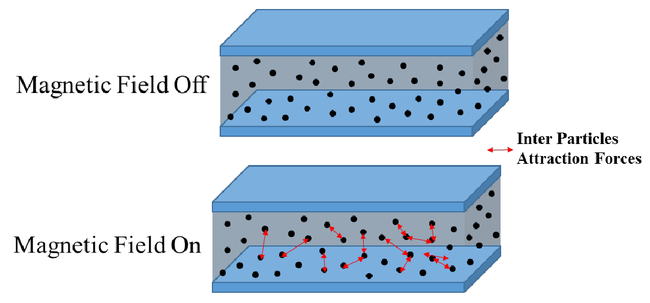
\includegraphics[width=0.6\linewidth]{Figures/MRE_actuate.jpg}
  \caption{Diagram showing MRE contraction actuation when a magnetic field is applied\citep{Park2018a}}
  \label{fig:Artificial Muscle_MRE}
\end{figure}
A key issue with using magnetorheological elastomers as soft actuators is that they require heavy gauge conductors for the high current they require for generating a magnetic field. The high current requirement means that actuators have only been created that have a solid electromagnet driving a soft MRE\citep{Bose2012}. 

When manufacturing MREs, uncured liquid silicone rubber is mixed with magnetic (commonly carbonyl iron) particles to form a 3 dimensional matrix of crosslinks with the magnetic particles fixed between the crosslinked polymers. A core issue when creating an MRE is the agglomeration and corrosion of magnetic particles due to residual water within the mixing operation. The magnetic particles can be processed to have a hydrophobic quality to mitigate this issue \cite{Burhannuddin2020,Ge2020}. During the curing process a magnetic field can be applied to align the particles within the elastomer to control the particle isotropy\cite{Ge2020,LaleganiDezaki2023}.

There have been attempts to use additive manufacturing to make MREs\citep{Krueger2014,Ge2020}, however the method described has not optimsied the structure of MRE for any application and the particle dipersion throughout the MRE has not been proven uniform throughout the print volume.

The current applications of MRE actuators are limited, however magnetorheological fluid (MRF), is a fluid which becomes more viscous with an applied magnetic field as currently has many modern applications. This fluid substance is largely used in applications where damping control is desired such as vehicle suspension\citep{UnuhH2019}, medical assitive devices\citep{Chen2017} and helicopter seat damping \citep{Hiemenz2007}. Potential MRE actuator applications include fluid valve control\citep{Bose2012} and active vibration control similar to that mentioned for MRFs\citep{UnuhH2019}.



\section{Soft Conductive Particle Piezoresistive Composites}
\label{sec:Soft Piezoresistive Composites}
% Why are soft piezo resistive composites used in S&As?
Soft sensors and actuators require low-stiffness materials for their active sensing/actuation domains. The requirement of softness is governed by the mechanical modulus values depend on the application requirements. The use of conductive particle elastomer composites is explored in this work due to the customisability of the electromechanical characteristics.
% Why CPECs
A core part of this thesis is understanding the behaviour of conductive particle elastomer composites for their use as a range of EAP-based sensing and actuating devices. The characteristics that make conductive particle elastomer composites (CPECs) ideal for soft sensor and actuator devices often include, low stiffness, controllable conductivity, controllable piezoresistivity, mouldable, 3D printable, low toxicity, durable, inexpensive, easy to obtain, simple fabrication process, and sustainable\cite{Chung2020,Ge2020,HindermannBischoff2001,Kim2012}.

\subsection{Fabricating Conductive Particle Elastomer Composites}
\label{subsec:Fabricating Conductive Particle Elastomer Composites}
Before exploring the known conduction and piezoresistive mechanisms and models for CPECs, it is important to understand how the fabrication process of a CPEC may affect its physical structure. 

CPECs are made by dispersing conductive particles through a curable liquid elastomer matrix. To change the electromechanical properties of the material, the dispersion of the conductive particles throughout the matrix can be optimised through various methods. To minimise the agglomerations of primary conductive particles often a sonication step is completed. This involves a mixture of the conductive particles and a liquid, usually in the form of a solvent, to be placed in a ultra-sonication bath. 

The sonication bath performs a frequency sweep and it has been shown that sudden implosion cavitation near the agglomerates help cause the separation of the agglomerates into their primary particles\cite{Priyadarshi2021,Kudryashova2019}. The degree of deagglomeration and dispersion is affected by various factors including sonciation time, frequency of oscillations, oscillation intensity, particle wettability, and liquid matrix viscosity\cite{Kudryashova2019,Chen2020a}. 

This sonication usually occurs before the the particles are added to the elastomeric matrix due to the large viscous damping effects of liquid elastomers. The next step involves mixing the dispersed conductive particles throughout the liquid elastomer, this can be done using a variety of mixing methods, including a planetary mixer, magnetic mixer, screw mixer, static mixers, amongst others \cite{Pegel2008,Rosset2016,Fekiri2020,Kim2012}. During the mixing process often the liquid solvent used in the dispersion stage is evaporated, leaving only the curable elastomer and the conductive particles. Although often impurities and voids are a by-product of the previous processes which can give undesirable qualities.

When sufficient mixing of the liquid elastomer and conductive particles have been completed the material is formed into a desired final shape using advanced additive manufacturing methods \cite{Bastola2018,Sapra2023,Krueger2014,Li2020,McCoul2017,Yi2023,Kim2018a} or traditional moulding \cite{Kim2018} or film making techniques \cite{Fasolt2017}. During the moulding process the material undergoes a form of curing, such as UV, catalysed, or moisture curing. If the composite material has not already been integrated into a device containing electrodes and other mechanical support structures these are integrated at the end of the process.


\subsection{Conductive Particle Elastomer Conduction Mechanisms}
Depending on the fabrication process stages stated in Section \ref{subsec:Fabricating Conductive Particle Elastomer Composites} for fabricating CPECs, the dispersion of conductive particles will always vary. 

\begin{figure}[H]
    \centering
    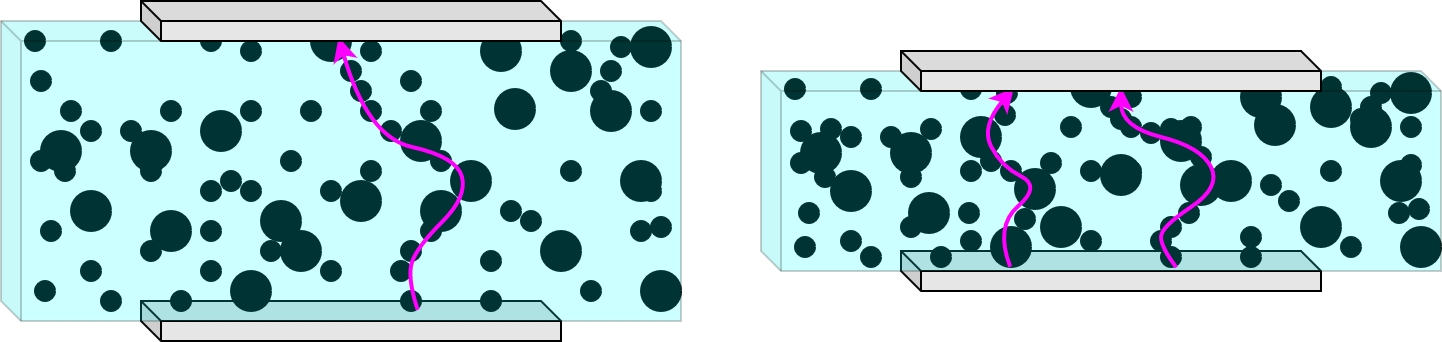
\includegraphics[width=0.7\linewidth]{Figures/res_deformed_states_x2_crop.jpg}
    \caption{Two grey highly conductive electrodes across a CPEC cuboid showing enlarged black conductive particles within a blue polymer matrix. Left: An uncompressed CPEC. Right: A compressed CPEC.}
    \label{fig:res_deformed_cube}
\end{figure}

Some of the physical features of these conductive percolation networks can be quantified and directly relate to the macro-level electromechanical properties of the material. Such characteristics of a conductive percolation network include, the type of conductive particle(s) used, particle dispersion, the elastomeric matrix, and any impurities or voids. The aspect ratio of a conductive particle filler can drastically change the conductivity and piezoresistivity of a CPEC. For example the aspect ratio of carbon nanotube particles (CNTs) is very large compared to that of regular carbon black (CB) particles, this has been shown to give improved conductivity for smaller weight volume percentages\cite{Wu2019,Flandin1999}, among other electromechanical property changes. Also the inherent particle conductivity a core parameter to consider when choosing a conductive particle composite.

Conductive particle dispersion is an important characterstic of CPECs when optimising the electrical properties of a CPEC. Particle dispersion includes the inter-particle distance distribution\cite{Kim2012}, particle agglomeration distribution\cite{Pegel2008}, particle isotropy/anisotropy \cite{Song2022}, and sedimentation\cite{Eklund2019}. The filler elastomer matrix also contributes to the piezoresistive effect, through it's viscoelasticity, elastic modulus, and dielectric permittivity within the CPEC.

% To do: Mention voids and impurities

\begin{figure}[H]
    \centering
    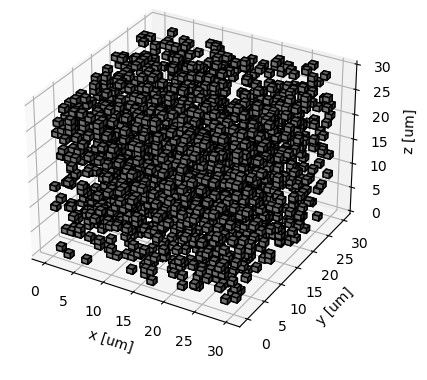
\includegraphics[width=0.6\linewidth]{Figures/simple_random_percolation.jpg}
    \caption{Example of a randomised cube percolation with a volume percentage of 8\% of particles}
    \label{fig:simp_rand_perc}
\end{figure}

% How you can model CBSR type material and the conduction mechanisms
Microscale models for CPECs and the relationship between particle and electric charge motion are often computationally heavy, overly idealised, and non-invertible \cite{Wang2022}. A microscale model example can be seen in Figure \ref{fig:simp_rand_perc}. However, microscale modelling of CPECs may give insight into understanding complex physical phenomena that may relate to the macroscale models made for CPECs. An alternate method for modelling CPECs is the formation of macroscale models\cite{Neffati2019}.

Electrical DC conduction through a CPEC occurs via two main mechanisms, Coulomb conduction and quantum tunneling \cite{Bloor2006,Duan2014,Zhang2007,Madrid2017}. Coulomb conduction uses the conduction band electrons are shared by adjacent atoms allow conduction throughout chains of cascading conductive particles. The second mechanism of conduction is through quantum tunneling which is stochastic in nature and allows for conduction through insulative boundaries between the percolative network of conductive particles \cite{Hu2008,Grimaldi2006}. 

Electrical AC conduction can occur through a CPEC through capacitive means depending of particle spacing with a decrease in reactance becoming more prominent for composites near the percolation threshold\cite{HindermannBischoff2001}.

% What have I contributed to the modelling of CBSR composites?
\newpage
\section{Literature Review Conclusions}
% Summarise: biological skin, artificial skin, biological muscle, artificial muscle, electroactive polymers.
% Clarify: the focus of the thesis.
The original purpose of this thesis was to develop novel sensor and actuator technology that mimics the pressure mapping capabilities of human skin and combine this with the actuation properties of human muscle. Through this review of current literature, several key conclusions can be drawn that will lay the foundational knowledge for the rest of this work.

The review of biological skin has revealed quantitative parameters that define its mechanical and sensory capabilities. This review highlighted mechanical characteristics such as the elastic modulus, viscoelastic creep, and surface area, as well as functional properties like spatial and temporal resolution. These factors provide a foundation for designing artificial skin that can replicate or even surpass the sensing functions of soft human skin. The review on pressure mapping technologies was then completed showing a range of different transduction methods for similarly soft sensing domains, showing that replicating human mechanoreceptor sensation is a multifaceted problem. Human skin uses various mechanoreceptors with different qualities and trade-offs and similarly different pressure mapping technologies use different pressure transduction methods each with different performance characteristics and limitations. The parallel review on biological and artificial muscles showed that DEAs and HASEL actuators are promising technologies for mimicking biological muscle quantitatively. Although characteristics common to both technologies such as high actuation voltage and limited device lifetime limit the applications of them.

The thesis has converged on using CPECs to fabricate EAP sensor and actuator devices, hence a brief literature review highlighting CPEC fabrication techniques and electromechanical characterisation has been given. These composites exhibit beneficial properties like flexibility, tunable electromechanical behavior, and ease of fabrication, which make them suitable for integrating into soft robotic systems. However, challenges such as achieving uniform particle dispersion, minimising agglomeration, and optimising the conductive network for stable long-term operation are still active areas of investigation.

This literature review has given a brief overview of some of the devices and theory related to the thesis, throughout the thesis there will be more background theory given on a need-to-know basis for each chapter.
% Excite: the reader into wanting to read the rest of the thesis!


%\section{Natural World Equivalents}
%\label{sec:Natural World Equivalents?}
% Find cases where DEAs, EIT, and EFT are seen in nature! Or a VERY close analogue to really push the importance of this work.

% from ReynoldsSmith1999 -> Many species of fish use electric fields to perceive their environments. The capability has evolved independently more than once: species in two distantly related families of fish, Mormyriformes and Gymnotoidei, one from South America and one from Africa, have this capability. This split is reflected in Figure 1-1, a family tree" of the fish known to have electrosensory capabilities. The fact that electric eld sensing does not require an external light source and is unaffected by optical scatterers like mud or silt is presumably advantageous to fish in dark, murky water anywhere. Electric Field sensing is another example of convergent evolution, the best known example being the eye, which evolved independently in squid and mammals. 
%In all examples of fish electric field sensing, a current source in the tail induces voltages along the lateral line. As the sh nears an ob ject with a dielectric constant dfferent than  water, the induced voltages change. Figure 1-2 shows the electric...